\section[Implementing a long-term planning tool for the natural gas transportation network]{Implementing a long-term planning tool for the natural gas transportation network}

\begin{frame}{One-day-ahead Models Forecasting}
	
	% This file was created with tikzplotlib v0.10.1.
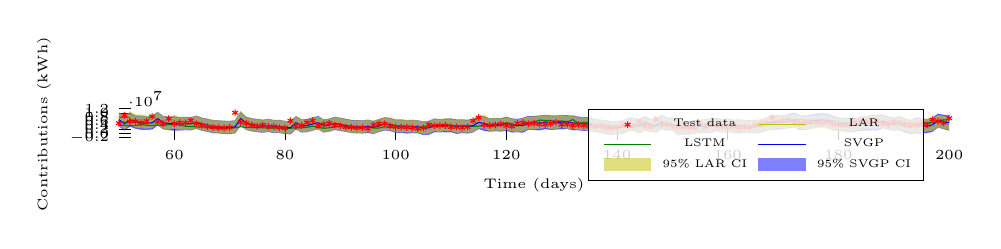
\begin{tikzpicture}

\definecolor{darkgray176}{RGB}{176,176,176}
\definecolor{goldenrod1911910}{RGB}{191,191,0}
\definecolor{green01270}{RGB}{0,127,0}
\definecolor{steelblue31119180}{RGB}{31,119,180}
\definecolor{lightgray204}{RGB}{204,204,204}
\definecolor{steelblue76114176}{RGB}{76,114,176}

\begin{axis}[
	width=\textwidth,
	height=2cm,
	axis line style={white},
	tick align=inside,
	tick pos=left,
	xlabel={Time (days)},
	xlabel style={font=\tiny},
	ylabel={Contributions (kWh)},
	ylabel style={font=\tiny},
	x grid style={white},
	xmajorgrids,
	xmin=50, xmax=200,
	xtick style={color=black},
	y grid style={white},
	ymajorgrids,
	ymin=-3414130.1187411, ymax=12497779.277438,
	ytick style={color=black},
	ytick={-4000000,-2000000,0,2000000,4000000,6000000,8000000,10000000,12000000,14000000},
	yticklabels={\ensuremath{-}\tiny0.4,\ensuremath{-}\tiny0.2,\tiny0.0,\tiny0.2,\tiny0.4,\tiny0.6,\tiny0.8,\tiny1.0,\tiny1.2,\tiny1.4},
	tick label style={font=\tiny},  % For all tick labels
	legend columns=2, 
	legend style={
		nodes={scale=0.8, transform shape},
		font=\tiny,
		fill opacity=0.8,
		draw opacity=1,
		text opacity=1,
		at={(0.03,0.97)},
		anchor=north west,
		legend pos=north east,
	},
]

\path [draw=blue, fill=blue, opacity=0.5]
(axis cs:0,8358734.9454699)
--(axis cs:0,2266980.59308182)
--(axis cs:1,2500001.54965498)
--(axis cs:2,2820173.30462753)
--(axis cs:3,2415130.35524611)
--(axis cs:4,2278827.62176907)
--(axis cs:5,2800080.67146894)
--(axis cs:6,2522735.91826576)
--(axis cs:7,2327115.22470213)
--(axis cs:8,1733100.31528789)
--(axis cs:9,2238909.43945783)
--(axis cs:10,1588035.67664878)
--(axis cs:11,1417358.47856748)
--(axis cs:12,1115298.76632328)
--(axis cs:13,3908825.52055853)
--(axis cs:14,3900131.47830728)
--(axis cs:15,2404535.30116041)
--(axis cs:16,155708.276391005)
--(axis cs:17,2546118.45607269)
--(axis cs:18,2497686.88060658)
--(axis cs:19,2224946.32585587)
--(axis cs:20,3528522.20106472)
--(axis cs:21,2993876.15193917)
--(axis cs:22,3512549.70941467)
--(axis cs:23,2491781.3003113)
--(axis cs:24,2328855.36877622)
--(axis cs:25,1586151.8126521)
--(axis cs:26,1631755.11754632)
--(axis cs:27,1304258.53410548)
--(axis cs:28,1440299.45566472)
--(axis cs:29,2524334.93887751)
--(axis cs:30,1469131.98383735)
--(axis cs:31,844807.886388455)
--(axis cs:32,1306990.45454863)
--(axis cs:33,1656600.4465597)
--(axis cs:34,1108728.6401974)
--(axis cs:35,1291186.74278974)
--(axis cs:36,1264438.19468078)
--(axis cs:37,3058834.81191941)
--(axis cs:38,3164334.38303838)
--(axis cs:39,2162251.43842642)
--(axis cs:40,2410788.57450276)
--(axis cs:41,1847879.46029119)
--(axis cs:42,3957465.21832349)
--(axis cs:43,2602714.55220306)
--(axis cs:44,1722471.05480101)
--(axis cs:45,3241330.05557888)
--(axis cs:46,3288785.66842647)
--(axis cs:47,2601220.79107986)
--(axis cs:48,2394130.4063376)
--(axis cs:49,1607416.13500269)
--(axis cs:50,3800571.8097075)
--(axis cs:51,1769959.66139186)
--(axis cs:52,3592891.04255399)
--(axis cs:53,2577387.46122187)
--(axis cs:54,2068056.39577527)
--(axis cs:55,2024187.16530619)
--(axis cs:56,2168232.03394953)
--(axis cs:57,4219749.91708765)
--(axis cs:58,2321099.19867304)
--(axis cs:59,1852980.63126997)
--(axis cs:60,1666742.29949185)
--(axis cs:61,1700757.83380629)
--(axis cs:62,1900526.36246136)
--(axis cs:63,1784170.84665271)
--(axis cs:64,2525056.64066475)
--(axis cs:65,1561832.5090252)
--(axis cs:66,1053349.26543152)
--(axis cs:67,414485.164985116)
--(axis cs:68,298119.463266004)
--(axis cs:69,81439.3687783941)
--(axis cs:70,-7820.22808993002)
--(axis cs:71,335716.133777275)
--(axis cs:72,4334340.95105938)
--(axis cs:73,1975368.907392)
--(axis cs:74,1288753.12099354)
--(axis cs:75,916344.071282642)
--(axis cs:76,614142.251991577)
--(axis cs:77,1010700.66828775)
--(axis cs:78,461598.17653731)
--(axis cs:79,494501.27675118)
--(axis cs:80,33830.2601246634)
--(axis cs:81,-125567.992846652)
--(axis cs:82,2292069.20046795)
--(axis cs:83,741536.54416309)
--(axis cs:84,919260.944394582)
--(axis cs:85,1658148.94372008)
--(axis cs:86,2302628.50777294)
--(axis cs:87,734480.659289974)
--(axis cs:88,1151364.96245121)
--(axis cs:89,1949088.1892057)
--(axis cs:90,1469898.3748664)
--(axis cs:91,1012199.53992729)
--(axis cs:92,506558.173343586)
--(axis cs:93,337040.472277472)
--(axis cs:94,276181.641666047)
--(axis cs:95,484026.183094725)
--(axis cs:96,53265.2106184359)
--(axis cs:97,979068.968634035)
--(axis cs:98,1723205.76503754)
--(axis cs:99,1479334.21275908)
--(axis cs:100,583871.637923067)
--(axis cs:101,634389.317676129)
--(axis cs:102,215739.931366092)
--(axis cs:103,461739.586981704)
--(axis cs:104,328907.277535586)
--(axis cs:105,-450025.291912541)
--(axis cs:106,-339424.825349538)
--(axis cs:107,859192.193391122)
--(axis cs:108,801036.768157851)
--(axis cs:109,879276.165044384)
--(axis cs:110,880185.232878993)
--(axis cs:111,83383.2972105495)
--(axis cs:112,485151.834711212)
--(axis cs:113,227653.60131191)
--(axis cs:114,810008.874069124)
--(axis cs:115,2435962.86066402)
--(axis cs:116,1538554.12054827)
--(axis cs:117,1131211.72805989)
--(axis cs:118,1356469.14897479)
--(axis cs:119,1207688.63023351)
--(axis cs:120,1552624.63758814)
--(axis cs:121,750359.686908945)
--(axis cs:122,834920.723187054)
--(axis cs:123,697240.26438279)
--(axis cs:124,2102986.1760763)
--(axis cs:125,1996251.22333412)
--(axis cs:126,1756514.14866896)
--(axis cs:127,2360006.57300085)
--(axis cs:128,1993913.19972267)
--(axis cs:129,2157217.91113449)
--(axis cs:130,2316694.30307414)
--(axis cs:131,2394260.09821298)
--(axis cs:132,1848239.17522981)
--(axis cs:133,1767530.89193186)
--(axis cs:134,1540891.21368726)
--(axis cs:135,1462010.18522907)
--(axis cs:136,861297.122579759)
--(axis cs:137,499864.711641925)
--(axis cs:138,-25725.608807263)
--(axis cs:139,-406884.282031849)
--(axis cs:140,-145638.354157871)
--(axis cs:141,134462.892064548)
--(axis cs:142,1348217.08221783)
--(axis cs:143,1479156.2743899)
--(axis cs:144,409275.546300376)
--(axis cs:145,1753441.01561209)
--(axis cs:146,997709.586344555)
--(axis cs:147,570250.159693988)
--(axis cs:148,2432273.85850153)
--(axis cs:149,1534298.14284645)
--(axis cs:150,1577962.02326722)
--(axis cs:151,-574621.177977669)
--(axis cs:152,-183460.994656229)
--(axis cs:153,-261513.429322622)
--(axis cs:154,267649.411942101)
--(axis cs:155,426525.009177709)
--(axis cs:156,570794.146962562)
--(axis cs:157,515871.19444223)
--(axis cs:158,1517382.94619805)
--(axis cs:159,666457.620843957)
--(axis cs:160,1079511.29250439)
--(axis cs:161,607435.347219682)
--(axis cs:162,358485.083181219)
--(axis cs:163,500307.141995887)
--(axis cs:164,487256.966723348)
--(axis cs:165,336996.194720265)
--(axis cs:166,746804.763099345)
--(axis cs:167,1639140.8386245)
--(axis cs:168,2086703.60388984)
--(axis cs:169,2082296.8180802)
--(axis cs:170,2421274.40362573)
--(axis cs:171,2743522.38725703)
--(axis cs:172,3276952.43104429)
--(axis cs:173,1893201.51116063)
--(axis cs:174,1888307.694171)
--(axis cs:175,2564733.61844642)
--(axis cs:176,3201720.08254982)
--(axis cs:177,3383492.24133263)
--(axis cs:178,3247965.71739236)
--(axis cs:179,1653295.63050552)
--(axis cs:180,1420123.69970278)
--(axis cs:181,1321184.89725323)
--(axis cs:182,840604.350411191)
--(axis cs:183,1069709.64984309)
--(axis cs:184,1605780.92757281)
--(axis cs:185,1461822.51297478)
--(axis cs:186,1760629.58786419)
--(axis cs:187,1684856.02697393)
--(axis cs:188,2869595.72832046)
--(axis cs:189,2112473.41992301)
--(axis cs:190,1601863.24076729)
--(axis cs:191,1992571.96940611)
--(axis cs:192,848324.710534492)
--(axis cs:193,-34180.7473299894)
--(axis cs:194,242736.46683395)
--(axis cs:195,320180.542585816)
--(axis cs:196,475112.983168926)
--(axis cs:197,1087350.75172669)
--(axis cs:198,3160250.31426845)
--(axis cs:199,2382899.974148)
--(axis cs:200,1682140.94545173)
--(axis cs:201,1192912.30192668)
--(axis cs:202,2443137.21793836)
--(axis cs:203,3056127.80714893)
--(axis cs:204,3464478.21770381)
--(axis cs:205,1593099.80141614)
--(axis cs:206,2065889.93122398)
--(axis cs:207,1682920.59535471)
--(axis cs:208,3106973.91932809)
--(axis cs:209,2797191.95707892)
--(axis cs:210,2775364.23799069)
--(axis cs:211,1089991.35094045)
--(axis cs:212,1367380.11977648)
--(axis cs:213,820132.807942717)
--(axis cs:214,1395607.06963896)
--(axis cs:215,1597109.15916967)
--(axis cs:216,2324573.18023901)
--(axis cs:217,944706.71099841)
--(axis cs:218,448713.343418519)
--(axis cs:219,-64693.0358876893)
--(axis cs:220,-29204.8480632002)
--(axis cs:221,240341.094173773)
--(axis cs:222,-281918.987639748)
--(axis cs:223,782429.004471717)
--(axis cs:224,521047.354232991)
--(axis cs:225,2345194.14055737)
--(axis cs:226,1368132.63085664)
--(axis cs:227,1230991.94258766)
--(axis cs:228,611057.273470148)
--(axis cs:229,77204.2095062481)
--(axis cs:230,-703629.858866641)
--(axis cs:231,-568034.528975812)
--(axis cs:232,-618345.175514996)
--(axis cs:233,-261129.287755128)
--(axis cs:234,-330004.860701131)
--(axis cs:235,-629314.936891818)
--(axis cs:236,-849909.293658883)
--(axis cs:237,-862056.450460804)
--(axis cs:238,-1491479.62577631)
--(axis cs:239,-1205160.6270297)
--(axis cs:240,-1236502.82817937)
--(axis cs:241,-421657.747989412)
--(axis cs:242,-1423787.05278457)
--(axis cs:243,-1727855.67463412)
--(axis cs:244,-1598521.89810558)
--(axis cs:245,-1384421.17327104)
--(axis cs:246,-1647104.77201385)
--(axis cs:247,-738046.085897258)
--(axis cs:248,-1504644.1046588)
--(axis cs:249,-1411386.36475813)
--(axis cs:250,-1403729.74361189)
--(axis cs:251,-1753899.81215703)
--(axis cs:252,-1549664.37286907)
--(axis cs:253,-1527701.31484671)
--(axis cs:254,-1362069.49284841)
--(axis cs:255,-1150810.85721608)
--(axis cs:256,-1263813.85555845)
--(axis cs:257,-668997.20244717)
--(axis cs:258,-1376281.03749657)
--(axis cs:259,-1087811.89019368)
--(axis cs:260,-1792309.2243679)
--(axis cs:261,-1917762.69837502)
--(axis cs:262,-1805955.64995552)
--(axis cs:263,-2260570.46921006)
--(axis cs:264,-1737120.45891163)
--(axis cs:265,-2032940.50447617)
--(axis cs:266,-1994001.01461112)
--(axis cs:267,-2028487.78775041)
--(axis cs:268,-1876425.76046569)
--(axis cs:269,-1291257.29209179)
--(axis cs:270,-648339.275730376)
--(axis cs:271,-1414311.32024024)
--(axis cs:272,-1754111.68023554)
--(axis cs:273,15785.7347802464)
--(axis cs:274,-346974.721788103)
--(axis cs:275,1295901.9458233)
--(axis cs:276,1280049.25219146)
--(axis cs:277,3091769.23677594)
--(axis cs:278,478672.307735468)
--(axis cs:279,395121.886578801)
--(axis cs:280,1636651.53361617)
--(axis cs:281,2575452.65146408)
--(axis cs:282,1469880.05512509)
--(axis cs:283,409829.911913471)
--(axis cs:284,631886.887580078)
--(axis cs:285,1893459.51588553)
--(axis cs:286,1368747.82714392)
--(axis cs:287,2407299.04277756)
--(axis cs:288,1390231.15819764)
--(axis cs:289,845028.71176875)
--(axis cs:290,1078146.57392484)
--(axis cs:291,972736.009060407)
--(axis cs:292,2992084.14802539)
--(axis cs:293,1966899.24784066)
--(axis cs:294,1582957.82595676)
--(axis cs:295,840697.009995176)
--(axis cs:296,570127.448758581)
--(axis cs:297,397552.276297163)
--(axis cs:298,1586229.90271889)
--(axis cs:299,938523.394328011)
--(axis cs:300,1637042.45551103)
--(axis cs:301,914360.994266017)
--(axis cs:302,102882.752574615)
--(axis cs:303,-393332.32100678)
--(axis cs:304,-424121.266243435)
--(axis cs:305,-289170.393837035)
--(axis cs:306,238565.073043851)
--(axis cs:307,791733.052337766)
--(axis cs:308,-38829.974295829)
--(axis cs:309,-545955.758686787)
--(axis cs:310,-586167.017135648)
--(axis cs:311,-442755.470135127)
--(axis cs:312,-531960.643466798)
--(axis cs:313,676124.109715074)
--(axis cs:314,-482649.734332843)
--(axis cs:315,1038283.73788468)
--(axis cs:316,205623.613565952)
--(axis cs:317,-381544.513242999)
--(axis cs:318,-406899.261562913)
--(axis cs:319,-284535.667012632)
--(axis cs:320,-286305.34626342)
--(axis cs:321,-346316.139303518)
--(axis cs:322,1040410.23285963)
--(axis cs:323,589404.961613129)
--(axis cs:324,707913.640332953)
--(axis cs:325,771388.936261653)
--(axis cs:326,595756.507183571)
--(axis cs:327,1054199.78227143)
--(axis cs:328,-305803.963151428)
--(axis cs:329,-593837.554806351)
--(axis cs:330,782481.948940561)
--(axis cs:331,1365746.26804607)
--(axis cs:332,958640.839148703)
--(axis cs:333,2339132.88508022)
--(axis cs:334,1050245.55835239)
--(axis cs:335,1221166.38615646)
--(axis cs:336,1195115.99955142)
--(axis cs:337,1096576.70209503)
--(axis cs:338,124977.524378125)
--(axis cs:339,965167.867562695)
--(axis cs:340,946780.992962114)
--(axis cs:341,739002.977938325)
--(axis cs:342,181450.554034516)
--(axis cs:343,139619.759726186)
--(axis cs:344,1085985.43091181)
--(axis cs:345,1146123.74095834)
--(axis cs:346,812329.486530669)
--(axis cs:347,641654.079815982)
--(axis cs:348,1217153.43036141)
--(axis cs:349,2473295.74536918)
--(axis cs:350,1314982.34765331)
--(axis cs:351,1772772.7666509)
--(axis cs:352,1215612.15422667)
--(axis cs:353,2146959.95908049)
--(axis cs:354,1837210.0040028)
--(axis cs:355,2033462.32888738)
--(axis cs:356,1980010.05607892)
--(axis cs:357,3039414.06621217)
--(axis cs:358,1863881.29906812)
--(axis cs:359,1531237.77681536)
--(axis cs:360,1207145.45452158)
--(axis cs:361,1224623.29228109)
--(axis cs:362,1742385.07182669)
--(axis cs:363,2904790.43576386)
--(axis cs:364,2547719.0813286)
--(axis cs:365,2854339.44720298)
--(axis cs:366,1257049.88256602)
--(axis cs:367,1870755.24321553)
--(axis cs:368,2614474.04894225)
--(axis cs:369,1588831.44143394)
--(axis cs:370,2360313.84061642)
--(axis cs:371,2401318.17182898)
--(axis cs:372,3064833.4140743)
--(axis cs:373,3192050.70963895)
--(axis cs:374,2663007.27200022)
--(axis cs:375,3709118.23830217)
--(axis cs:376,2335728.38327879)
--(axis cs:377,4025739.01063027)
--(axis cs:378,4055408.83132899)
--(axis cs:379,2960992.68942342)
--(axis cs:380,2657390.42843395)
--(axis cs:381,2722234.42908046)
--(axis cs:382,3103809.54765794)
--(axis cs:383,3272887.22177995)
--(axis cs:384,2741714.33565594)
--(axis cs:385,3707114.31719387)
--(axis cs:386,3515979.43874086)
--(axis cs:387,2687537.20342327)
--(axis cs:388,2840202.86134352)
--(axis cs:389,3053290.7891614)
--(axis cs:390,2624280.63959711)
--(axis cs:391,1996525.2894387)
--(axis cs:392,3987152.74982535)
--(axis cs:393,3488735.45628922)
--(axis cs:394,4859209.60018155)
--(axis cs:395,3785810.63864612)
--(axis cs:396,2651825.09161797)
--(axis cs:397,2342689.32647771)
--(axis cs:398,1724308.38006152)
--(axis cs:399,3116503.58527372)
--(axis cs:400,2713962.51998371)
--(axis cs:401,2924991.8355552)
--(axis cs:402,1759784.98522933)
--(axis cs:403,2663118.2481602)
--(axis cs:404,4544813.79217867)
--(axis cs:405,5064879.7229684)
--(axis cs:406,3647294.34128199)
--(axis cs:407,2477553.36206289)
--(axis cs:408,2357641.3363899)
--(axis cs:409,3691593.57461331)
--(axis cs:410,2712420.65312779)
--(axis cs:411,2180599.51772762)
--(axis cs:412,3085656.53750853)
--(axis cs:413,2915976.19105762)
--(axis cs:414,3075394.13093566)
--(axis cs:415,3303878.67127666)
--(axis cs:416,2288488.00111913)
--(axis cs:417,1884126.24464031)
--(axis cs:418,1562775.86596284)
--(axis cs:419,1670034.05930531)
--(axis cs:420,1330120.0918032)
--(axis cs:421,1245506.03135283)
--(axis cs:422,1139180.17608696)
--(axis cs:423,1716689.00137541)
--(axis cs:424,1127174.99347224)
--(axis cs:425,920644.833256553)
--(axis cs:426,833019.426799105)
--(axis cs:427,977829.022656063)
--(axis cs:428,573895.003956363)
--(axis cs:429,304425.050964801)
--(axis cs:430,385634.028432807)
--(axis cs:431,3170498.39166676)
--(axis cs:432,1269443.10069475)
--(axis cs:433,582683.241494185)
--(axis cs:434,338342.607890409)
--(axis cs:435,198134.636922647)
--(axis cs:436,3700128.99467785)
--(axis cs:437,3708934.5229381)
--(axis cs:438,2126149.2257448)
--(axis cs:439,3653330.29513892)
--(axis cs:440,2375245.67171627)
--(axis cs:440,8272115.97564292)
--(axis cs:440,8272115.97564292)
--(axis cs:439,10011577.5456571)
--(axis cs:438,7997611.41757856)
--(axis cs:437,9635565.99844665)
--(axis cs:436,9607828.31427181)
--(axis cs:435,6072861.77476716)
--(axis cs:434,6212873.20124285)
--(axis cs:433,6452280.79079365)
--(axis cs:432,7149477.70611468)
--(axis cs:431,9063394.31624093)
--(axis cs:430,6283774.64694488)
--(axis cs:429,6196312.25641046)
--(axis cs:428,6616585.42512907)
--(axis cs:427,6906795.03319433)
--(axis cs:426,6763781.61119613)
--(axis cs:425,7012796.19856471)
--(axis cs:424,7089689.32194692)
--(axis cs:423,7656594.18475407)
--(axis cs:422,7095689.9374345)
--(axis cs:421,7289410.08378023)
--(axis cs:420,7505021.90638861)
--(axis cs:419,7713792.59164026)
--(axis cs:418,7511894.8093766)
--(axis cs:417,7947574.99178663)
--(axis cs:416,8241270.69192941)
--(axis cs:415,9272062.72279752)
--(axis cs:414,9003539.46431187)
--(axis cs:413,8846613.44772675)
--(axis cs:412,9105367.22263592)
--(axis cs:411,8079776.77631247)
--(axis cs:410,8600197.55973165)
--(axis cs:409,9684244.9945811)
--(axis cs:408,8227475.4132527)
--(axis cs:407,8351959.65928155)
--(axis cs:406,9556521.83074564)
--(axis cs:405,11088718.651684)
--(axis cs:404,10562655.5164873)
--(axis cs:403,8677451.54084561)
--(axis cs:402,7724399.75366388)
--(axis cs:401,8900148.4912878)
--(axis cs:400,8619427.20856482)
--(axis cs:399,9023644.62626584)
--(axis cs:398,7654322.89644653)
--(axis cs:397,8325906.4041908)
--(axis cs:396,8854878.21402704)
--(axis cs:395,10134240.9070042)
--(axis cs:394,10942794.0012594)
--(axis cs:393,9412306.42744924)
--(axis cs:392,9890440.27644084)
--(axis cs:391,7862314.42334116)
--(axis cs:390,8539608.8276385)
--(axis cs:389,8943656.49523974)
--(axis cs:388,8749942.91793317)
--(axis cs:387,8705300.56734983)
--(axis cs:386,9451385.92980784)
--(axis cs:385,9661638.45024246)
--(axis cs:384,8800115.49330164)
--(axis cs:383,9329078.99326154)
--(axis cs:382,9119536.39494003)
--(axis cs:381,8711040.05201311)
--(axis cs:380,9049290.99227471)
--(axis cs:379,9504148.53201147)
--(axis cs:378,10410231.6107597)
--(axis cs:377,10326557.3212269)
--(axis cs:376,8728582.683576)
--(axis cs:375,9673920.17516636)
--(axis cs:374,8634933.11425413)
--(axis cs:373,9157477.21893432)
--(axis cs:372,9157929.60738453)
--(axis cs:371,8326286.22268122)
--(axis cs:370,8242256.81424885)
--(axis cs:369,7508145.32098696)
--(axis cs:368,8546925.55539232)
--(axis cs:367,7878369.78688992)
--(axis cs:366,7749147.7691826)
--(axis cs:365,8777805.04685025)
--(axis cs:364,8621207.45742553)
--(axis cs:363,8936822.6694143)
--(axis cs:362,8026606.42024076)
--(axis cs:361,7196783.10732654)
--(axis cs:360,7413401.58474042)
--(axis cs:359,7555906.77588987)
--(axis cs:358,8088401.43404874)
--(axis cs:357,9679920.01725985)
--(axis cs:356,8076758.88553188)
--(axis cs:355,8052209.41518265)
--(axis cs:354,7933664.42316086)
--(axis cs:353,8492570.42424654)
--(axis cs:352,7308779.19156219)
--(axis cs:351,7818817.95504795)
--(axis cs:350,7573739.38620749)
--(axis cs:349,8797907.06987265)
--(axis cs:348,7375941.65053311)
--(axis cs:347,6569846.35313213)
--(axis cs:346,6743196.52320619)
--(axis cs:345,7044621.54291345)
--(axis cs:344,7092701.77476335)
--(axis cs:343,6136173.89898583)
--(axis cs:342,6344575.61516148)
--(axis cs:341,6779463.28788147)
--(axis cs:340,6860105.47907654)
--(axis cs:339,6944443.82978215)
--(axis cs:338,6237386.42674522)
--(axis cs:337,7133470.37297508)
--(axis cs:336,7418021.26036287)
--(axis cs:335,7132481.80986207)
--(axis cs:334,6943400.89190936)
--(axis cs:333,8351541.70390249)
--(axis cs:332,6994699.02333084)
--(axis cs:331,7366236.27538514)
--(axis cs:330,6736401.87984606)
--(axis cs:329,5729913.61972009)
--(axis cs:328,6152138.0355138)
--(axis cs:327,7091179.723979)
--(axis cs:326,6587905.42111292)
--(axis cs:325,6741081.92349823)
--(axis cs:324,6927522.95220145)
--(axis cs:323,6732134.31011498)
--(axis cs:322,7414879.48424147)
--(axis cs:321,5646266.81566105)
--(axis cs:320,5639928.66468998)
--(axis cs:319,5611793.89013555)
--(axis cs:318,5520410.31099636)
--(axis cs:317,5557630.12102689)
--(axis cs:316,6317348.65003779)
--(axis cs:315,8133806.0487823)
--(axis cs:314,6271361.26806303)
--(axis cs:313,6926779.59231562)
--(axis cs:312,5351487.17626322)
--(axis cs:311,5487382.36968934)
--(axis cs:310,5293847.53066585)
--(axis cs:309,5313036.47539066)
--(axis cs:308,5836358.77445582)
--(axis cs:307,6806428.95975679)
--(axis cs:306,6145055.03764359)
--(axis cs:305,5597596.29577675)
--(axis cs:304,5615029.20658272)
--(axis cs:303,5746438.19449132)
--(axis cs:302,6044624.93079489)
--(axis cs:301,6883756.24313143)
--(axis cs:300,7717297.41396964)
--(axis cs:299,6999180.00143638)
--(axis cs:298,7722016.09685706)
--(axis cs:297,6500962.58968753)
--(axis cs:296,6439857.44289134)
--(axis cs:295,6708598.62648087)
--(axis cs:294,7544073.9674112)
--(axis cs:293,8101619.38663902)
--(axis cs:292,9116088.93195463)
--(axis cs:291,6989022.07507434)
--(axis cs:290,6970124.22981287)
--(axis cs:289,7056445.31115333)
--(axis cs:288,7295821.7252935)
--(axis cs:287,8376488.11238208)
--(axis cs:286,7578421.4232308)
--(axis cs:285,8046576.21229546)
--(axis cs:284,7212922.64090839)
--(axis cs:283,6521406.92841331)
--(axis cs:282,7554490.42794916)
--(axis cs:281,8681908.70211522)
--(axis cs:280,7858043.03039205)
--(axis cs:279,6922764.17147553)
--(axis cs:278,6880386.67496839)
--(axis cs:277,9146553.78321283)
--(axis cs:276,7379428.98116728)
--(axis cs:275,7513575.53765563)
--(axis cs:274,5741060.86128361)
--(axis cs:273,6170870.39527822)
--(axis cs:272,4412738.07280879)
--(axis cs:271,5125181.63389964)
--(axis cs:270,5279902.76289232)
--(axis cs:269,4601444.70584617)
--(axis cs:268,4004144.58825829)
--(axis cs:267,3867664.14440554)
--(axis cs:266,3918913.50021261)
--(axis cs:265,3901956.96393358)
--(axis cs:264,4429298.28023224)
--(axis cs:263,3685876.01529592)
--(axis cs:262,4107167.51973562)
--(axis cs:261,4092723.1457314)
--(axis cs:260,4970792.8097317)
--(axis cs:259,4907549.33909286)
--(axis cs:258,4562806.88204193)
--(axis cs:257,5564992.31940384)
--(axis cs:256,4742276.74049143)
--(axis cs:255,4977378.99761699)
--(axis cs:254,4934040.50236445)
--(axis cs:253,4875146.15793132)
--(axis cs:252,4849843.12505433)
--(axis cs:251,4591102.05855391)
--(axis cs:250,4680614.08481247)
--(axis cs:249,4806759.63655051)
--(axis cs:248,5398519.23058963)
--(axis cs:247,5924235.62056438)
--(axis cs:246,4577806.77403004)
--(axis cs:245,4562165.87791714)
--(axis cs:244,4419361.76158695)
--(axis cs:243,4519559.84972538)
--(axis cs:242,4903736.64106637)
--(axis cs:241,6474664.50268905)
--(axis cs:240,5034204.73774535)
--(axis cs:239,5203836.55271089)
--(axis cs:238,4889401.78115006)
--(axis cs:237,5028271.6617677)
--(axis cs:236,5030147.92350487)
--(axis cs:235,5249275.18224642)
--(axis cs:234,5540223.699851)
--(axis cs:233,5608686.81977924)
--(axis cs:232,5668616.25525784)
--(axis cs:231,5371440.13637239)
--(axis cs:230,5246016.17185683)
--(axis cs:229,6114481.1296214)
--(axis cs:228,6592394.04485644)
--(axis cs:227,7233892.55599388)
--(axis cs:226,7560745.16767292)
--(axis cs:225,8311358.80833407)
--(axis cs:224,7495803.994909)
--(axis cs:223,6878220.36672014)
--(axis cs:222,6160229.64507523)
--(axis cs:221,7318835.36975051)
--(axis cs:220,7246663.17516622)
--(axis cs:219,6615836.61209439)
--(axis cs:218,6749113.88839668)
--(axis cs:217,7107473.99710223)
--(axis cs:216,8555535.72940454)
--(axis cs:215,8367306.12768181)
--(axis cs:214,8095423.00720392)
--(axis cs:213,7694157.98714085)
--(axis cs:212,8323090.08105852)
--(axis cs:211,7995439.59566517)
--(axis cs:210,9045449.95771611)
--(axis cs:209,9564570.78842258)
--(axis cs:208,9821419.46295298)
--(axis cs:207,7837769.33742558)
--(axis cs:206,8255574.25607588)
--(axis cs:205,7849736.53431507)
--(axis cs:204,9576660.33798847)
--(axis cs:203,9368591.47472401)
--(axis cs:202,9165616.33649763)
--(axis cs:201,8390043.92014571)
--(axis cs:200,8607782.67335589)
--(axis cs:199,8799351.17919425)
--(axis cs:198,9357307.81325061)
--(axis cs:197,7483283.09942182)
--(axis cs:196,6683454.5725114)
--(axis cs:195,7053163.66442116)
--(axis cs:194,7565404.86683807)
--(axis cs:193,6200732.26408663)
--(axis cs:192,7171495.15083943)
--(axis cs:191,8203105.65223896)
--(axis cs:190,7498392.46651707)
--(axis cs:189,8076362.84351501)
--(axis cs:188,9058808.51068171)
--(axis cs:187,8821475.6751613)
--(axis cs:186,8751212.73423382)
--(axis cs:185,8118458.38378642)
--(axis cs:184,8124343.62316064)
--(axis cs:183,7007270.76272865)
--(axis cs:182,6940343.87525926)
--(axis cs:181,7304634.6108532)
--(axis cs:180,7564718.08769193)
--(axis cs:179,8328475.01770524)
--(axis cs:178,9485792.02733359)
--(axis cs:177,9689734.59750967)
--(axis cs:176,9450465.06717683)
--(axis cs:175,8948079.59175623)
--(axis cs:174,8405988.85831612)
--(axis cs:173,8741083.26570942)
--(axis cs:172,9968137.23215174)
--(axis cs:171,9126666.41570682)
--(axis cs:170,8496109.73289019)
--(axis cs:169,8829265.88352662)
--(axis cs:168,8360476.29898034)
--(axis cs:167,7651737.10059532)
--(axis cs:166,6754528.58466087)
--(axis cs:165,6221099.08431227)
--(axis cs:164,6336008.42282694)
--(axis cs:163,6390368.43425088)
--(axis cs:162,6606684.21313195)
--(axis cs:161,6463712.2109056)
--(axis cs:160,6971719.21072575)
--(axis cs:159,6527237.92416448)
--(axis cs:158,7448595.25540128)
--(axis cs:157,6552109.10429121)
--(axis cs:156,6876578.59679644)
--(axis cs:155,6361114.3912048)
--(axis cs:154,6338968.35592609)
--(axis cs:153,5743938.08214018)
--(axis cs:152,5713168.05937878)
--(axis cs:151,6009137.88882062)
--(axis cs:150,7517804.93430203)
--(axis cs:149,7453006.41713491)
--(axis cs:148,8823440.02242871)
--(axis cs:147,6479591.52044145)
--(axis cs:146,6995421.00812897)
--(axis cs:145,8233454.97190743)
--(axis cs:144,6713913.47421679)
--(axis cs:143,7439774.41928997)
--(axis cs:142,7368120.91903883)
--(axis cs:141,6110114.93413916)
--(axis cs:140,5835392.60034468)
--(axis cs:139,5645436.82020181)
--(axis cs:138,6216849.71122078)
--(axis cs:137,6512801.79719511)
--(axis cs:136,6822078.74304201)
--(axis cs:135,7626219.47830896)
--(axis cs:134,7767868.70129548)
--(axis cs:133,7887300.40473132)
--(axis cs:132,8530712.12434376)
--(axis cs:131,8585430.70651424)
--(axis cs:130,8687812.82110287)
--(axis cs:129,8496024.70025284)
--(axis cs:128,8534211.24710132)
--(axis cs:127,8780268.08636291)
--(axis cs:126,8507297.96736859)
--(axis cs:125,8257204.86348395)
--(axis cs:124,8315657.53908073)
--(axis cs:123,7344078.02207404)
--(axis cs:122,6861840.24356864)
--(axis cs:121,7104377.22877023)
--(axis cs:120,7926765.7469317)
--(axis cs:119,7186307.56303116)
--(axis cs:118,7331921.3006784)
--(axis cs:117,7054113.09715032)
--(axis cs:116,8036195.88384113)
--(axis cs:115,8400746.88129105)
--(axis cs:114,6767631.53735761)
--(axis cs:113,6489285.1899857)
--(axis cs:112,6572828.73970546)
--(axis cs:111,6589342.49793673)
--(axis cs:110,7050296.12744666)
--(axis cs:109,6941615.68986246)
--(axis cs:108,6727736.37519017)
--(axis cs:107,7032339.83230106)
--(axis cs:106,5942141.16199991)
--(axis cs:105,5580414.23217365)
--(axis cs:104,6196126.35290635)
--(axis cs:103,6369006.45094391)
--(axis cs:102,6243937.36821829)
--(axis cs:101,6552787.49936702)
--(axis cs:100,6543608.10188798)
--(axis cs:99,7382894.8860172)
--(axis cs:98,7622566.72894418)
--(axis cs:97,6838346.22382169)
--(axis cs:96,5920294.43025754)
--(axis cs:95,6441826.59383301)
--(axis cs:94,6149797.52850492)
--(axis cs:93,6206888.85275809)
--(axis cs:92,6388734.23595245)
--(axis cs:91,6884044.87736475)
--(axis cs:90,7411976.85666203)
--(axis cs:89,7850708.56649312)
--(axis cs:88,7005061.36887078)
--(axis cs:87,6580907.25089671)
--(axis cs:86,8170430.18127629)
--(axis cs:85,7688961.45795676)
--(axis cs:84,6789576.38948332)
--(axis cs:83,6587541.17027693)
--(axis cs:82,8163788.22862993)
--(axis cs:81,5728882.98666019)
--(axis cs:80,5881873.52566259)
--(axis cs:79,6346344.07212325)
--(axis cs:78,6322332.28316718)
--(axis cs:77,6868374.19837788)
--(axis cs:76,6467593.4559952)
--(axis cs:75,6790634.5611246)
--(axis cs:74,7189172.85758338)
--(axis cs:73,7845279.66202889)
--(axis cs:72,10309744.0530896)
--(axis cs:71,6181063.40738308)
--(axis cs:70,5873490.67430435)
--(axis cs:69,5942240.9806898)
--(axis cs:68,6151217.53147982)
--(axis cs:67,6281228.43259183)
--(axis cs:66,6921993.32150405)
--(axis cs:65,7430653.31981543)
--(axis cs:64,8406789.07029833)
--(axis cs:63,7678032.30836992)
--(axis cs:62,7779339.94755391)
--(axis cs:61,7691533.04200607)
--(axis cs:60,8118902.77594928)
--(axis cs:59,7888649.84230029)
--(axis cs:58,8231240.35421631)
--(axis cs:57,10225728.8837369)
--(axis cs:56,8284864.42376014)
--(axis cs:55,8056270.85700612)
--(axis cs:54,8188802.99412978)
--(axis cs:53,8587803.84291661)
--(axis cs:52,9757365.74140004)
--(axis cs:51,7774258.72978544)
--(axis cs:50,9773012.90077685)
--(axis cs:49,7543662.45878557)
--(axis cs:48,8366369.02485663)
--(axis cs:47,8527050.32973806)
--(axis cs:46,9288516.00961098)
--(axis cs:45,9215131.79049679)
--(axis cs:44,8465639.15914963)
--(axis cs:43,8848468.33443262)
--(axis cs:42,9975524.31028236)
--(axis cs:41,7716513.35888516)
--(axis cs:40,8585590.444903)
--(axis cs:39,8046697.65811915)
--(axis cs:38,9061277.56638082)
--(axis cs:37,8959598.76533762)
--(axis cs:36,7171564.90185334)
--(axis cs:35,7145907.04617949)
--(axis cs:34,6965455.88627264)
--(axis cs:33,7617839.5279707)
--(axis cs:32,7159094.12709909)
--(axis cs:31,6700804.58801861)
--(axis cs:30,7343517.78973181)
--(axis cs:29,8431175.26424769)
--(axis cs:28,7330522.14541852)
--(axis cs:27,7225547.45175696)
--(axis cs:26,7537979.7512287)
--(axis cs:25,7488757.26602932)
--(axis cs:24,8242394.44899235)
--(axis cs:23,8379204.91061556)
--(axis cs:22,9441647.08735033)
--(axis cs:21,9266193.03407906)
--(axis cs:20,9728685.25839887)
--(axis cs:19,8322686.81444134)
--(axis cs:18,8687097.44746864)
--(axis cs:17,8804705.0708452)
--(axis cs:16,7481962.56861928)
--(axis cs:15,8359167.58209611)
--(axis cs:14,9917343.03729903)
--(axis cs:13,9901265.5631022)
--(axis cs:12,7058300.0424605)
--(axis cs:11,7300393.23963672)
--(axis cs:10,7631033.41849808)
--(axis cs:9,8404156.88651083)
--(axis cs:8,8227013.51280867)
--(axis cs:7,8862452.77799191)
--(axis cs:6,9114397.94396872)
--(axis cs:5,9233470.8886454)
--(axis cs:4,9147653.1877756)
--(axis cs:3,8830004.51601952)
--(axis cs:2,9353245.08095938)
--(axis cs:1,9366401.36241324)
--(axis cs:0,8358734.9454699)
--cycle;

\path [draw=goldenrod1911910, fill=goldenrod1911910, opacity=0.5]
(axis cs:0,7649611.36140954)
--(axis cs:0,2031353.86694591)
--(axis cs:1,3519778.99023208)
--(axis cs:2,2939647.83093819)
--(axis cs:3,2404739.40901625)
--(axis cs:4,2599711.14663126)
--(axis cs:5,2663728.74643248)
--(axis cs:6,2426379.1016333)
--(axis cs:7,2232546.72630842)
--(axis cs:8,1668469.54697674)
--(axis cs:9,2057827.52360267)
--(axis cs:10,1490958.45797037)
--(axis cs:11,1185100.63458257)
--(axis cs:12,964716.243901049)
--(axis cs:13,3834280.95472574)
--(axis cs:14,4058426.74441934)
--(axis cs:15,2463915.32277849)
--(axis cs:16,1625007.40781802)
--(axis cs:17,2045788.16372025)
--(axis cs:18,2615535.96239301)
--(axis cs:19,2108399.57141996)
--(axis cs:20,4265001.05360169)
--(axis cs:21,3419640.3442961)
--(axis cs:22,3311831.70608119)
--(axis cs:23,2378382.24669818)
--(axis cs:24,2299225.49424298)
--(axis cs:25,1586672.89565133)
--(axis cs:26,1734188.38705589)
--(axis cs:27,1377097.6756055)
--(axis cs:28,1501859.3903355)
--(axis cs:29,2519230.24015983)
--(axis cs:30,1602768.89488034)
--(axis cs:31,994183.893438096)
--(axis cs:32,1383863.25026629)
--(axis cs:33,1846530.28765762)
--(axis cs:34,1239775.97277975)
--(axis cs:35,1394730.10840429)
--(axis cs:36,1388129.72336291)
--(axis cs:37,3212874.42384193)
--(axis cs:38,3250052.05093703)
--(axis cs:39,2212330.83063421)
--(axis cs:40,2988267.81816703)
--(axis cs:41,1940811.17360877)
--(axis cs:42,4501668.5981036)
--(axis cs:43,4362329.57020703)
--(axis cs:44,4774876.89487605)
--(axis cs:45,3761577.41166215)
--(axis cs:46,3833183.17858582)
--(axis cs:47,2941135.19156964)
--(axis cs:48,3050059.16855053)
--(axis cs:49,2065029.89060203)
--(axis cs:50,4500022.86644034)
--(axis cs:51,2272764.7465469)
--(axis cs:52,4794628.18392887)
--(axis cs:53,3185752.31783906)
--(axis cs:54,3393025.53630686)
--(axis cs:55,2763798.96680438)
--(axis cs:56,3090198.52648587)
--(axis cs:57,4515895.54251675)
--(axis cs:58,2597299.22762645)
--(axis cs:59,2047454.01280886)
--(axis cs:60,3077708.1641259)
--(axis cs:61,1923991.90230687)
--(axis cs:62,2023265.34145536)
--(axis cs:63,1945120.18593477)
--(axis cs:64,2671939.69385065)
--(axis cs:65,1712801.45250672)
--(axis cs:66,1257472.62148182)
--(axis cs:67,669374.331022673)
--(axis cs:68,525431.049548327)
--(axis cs:69,354030.832588086)
--(axis cs:70,223072.663671357)
--(axis cs:71,547211.055081147)
--(axis cs:72,4891812.83621656)
--(axis cs:73,1967492.40125675)
--(axis cs:74,1546038.27733403)
--(axis cs:75,995871.714654822)
--(axis cs:76,744308.887271639)
--(axis cs:77,1195718.70252183)
--(axis cs:78,664904.436480089)
--(axis cs:79,635419.536387467)
--(axis cs:80,269721.970536069)
--(axis cs:81,121292.406592703)
--(axis cs:82,2419182.85003434)
--(axis cs:83,818592.975010572)
--(axis cs:84,972004.782306544)
--(axis cs:85,1878727.1436674)
--(axis cs:86,2327387.28519245)
--(axis cs:87,909879.323522354)
--(axis cs:88,1265832.79529863)
--(axis cs:89,2068057.92654706)
--(axis cs:90,1703252.06764654)
--(axis cs:91,1113763.15278355)
--(axis cs:92,543285.504705829)
--(axis cs:93,464062.304703045)
--(axis cs:94,420561.625391634)
--(axis cs:95,970038.564103642)
--(axis cs:96,239762.295294122)
--(axis cs:97,1253147.13821133)
--(axis cs:98,1917151.5980573)
--(axis cs:99,1774552.46575942)
--(axis cs:100,776063.778164456)
--(axis cs:101,813515.709810239)
--(axis cs:102,786952.781699222)
--(axis cs:103,693673.769717739)
--(axis cs:104,561581.60775435)
--(axis cs:105,-9449.11910516536)
--(axis cs:106,140563.902805642)
--(axis cs:107,1390080.20385617)
--(axis cs:108,917707.095869979)
--(axis cs:109,1637776.6105716)
--(axis cs:110,1516861.73686869)
--(axis cs:111,522320.456940449)
--(axis cs:112,791543.269129801)
--(axis cs:113,485495.585377553)
--(axis cs:114,1006838.30867687)
--(axis cs:115,2629796.0113633)
--(axis cs:116,3068871.19888404)
--(axis cs:117,1353594.42178321)
--(axis cs:118,1607003.6062809)
--(axis cs:119,1418412.93529407)
--(axis cs:120,2019398.0635785)
--(axis cs:121,1276219.55230597)
--(axis cs:122,1022015.57819442)
--(axis cs:123,1444372.47035012)
--(axis cs:124,2383625.07692119)
--(axis cs:125,2458447.44376003)
--(axis cs:126,2747159.64731046)
--(axis cs:127,2986996.31238164)
--(axis cs:128,2553268.52467772)
--(axis cs:129,2492825.67459294)
--(axis cs:130,3042842.78513953)
--(axis cs:131,2546061.12872144)
--(axis cs:132,2597984.60251658)
--(axis cs:133,1932673.18498694)
--(axis cs:134,2094101.17897937)
--(axis cs:135,1346176.48957805)
--(axis cs:136,987586.951263016)
--(axis cs:137,728988.962961117)
--(axis cs:138,315617.909551716)
--(axis cs:139,-49323.9594325367)
--(axis cs:140,162905.198747895)
--(axis cs:141,311057.572960953)
--(axis cs:142,1387230.36566185)
--(axis cs:143,1348269.76838078)
--(axis cs:144,750080.14300655)
--(axis cs:145,2444127.25624494)
--(axis cs:146,1138002.5994334)
--(axis cs:147,679751.622814542)
--(axis cs:148,2974810.39345845)
--(axis cs:149,1418900.35584527)
--(axis cs:150,1478480.77640972)
--(axis cs:151,-519001.598609076)
--(axis cs:152,131269.34499085)
--(axis cs:153,128089.471677241)
--(axis cs:154,417721.873055306)
--(axis cs:155,363932.5014591)
--(axis cs:156,1267233.87220423)
--(axis cs:157,685848.911851416)
--(axis cs:158,1645838.61939955)
--(axis cs:159,775524.654280999)
--(axis cs:160,1294604.47446742)
--(axis cs:161,644049.660954553)
--(axis cs:162,792820.020044177)
--(axis cs:163,608584.097401883)
--(axis cs:164,577498.455183456)
--(axis cs:165,504896.293255964)
--(axis cs:166,1146833.98756396)
--(axis cs:167,1985793.60462994)
--(axis cs:168,2116297.44403296)
--(axis cs:169,2994417.42082804)
--(axis cs:170,2671225.79353657)
--(axis cs:171,2966003.82376621)
--(axis cs:172,3246303.12019177)
--(axis cs:173,2726520.99249482)
--(axis cs:174,2106448.68977005)
--(axis cs:175,2622418.68395817)
--(axis cs:176,2652163.34204217)
--(axis cs:177,2948967.62755043)
--(axis cs:178,2397655.79724452)
--(axis cs:179,1707984.7835188)
--(axis cs:180,1436666.45138223)
--(axis cs:181,1353787.23172246)
--(axis cs:182,1224416.35895755)
--(axis cs:183,1195041.31824965)
--(axis cs:184,2602578.08821537)
--(axis cs:185,2528445.76566443)
--(axis cs:186,2689870.39937288)
--(axis cs:187,2853066.33954884)
--(axis cs:188,3016441.35360949)
--(axis cs:189,2066114.2752357)
--(axis cs:190,1675601.58076407)
--(axis cs:191,2531910.75137634)
--(axis cs:192,1632952.49102099)
--(axis cs:193,1050371.95963481)
--(axis cs:194,486685.886614144)
--(axis cs:195,1005855.33288483)
--(axis cs:196,1336794.71128583)
--(axis cs:197,1630377.18719138)
--(axis cs:198,3069328.08431613)
--(axis cs:199,2594961.74965377)
--(axis cs:200,2034287.27493114)
--(axis cs:201,3404756.13163478)
--(axis cs:202,3681198.5215013)
--(axis cs:203,3660536.09196788)
--(axis cs:204,3296027.13161012)
--(axis cs:205,2310832.12801823)
--(axis cs:206,2245108.17031315)
--(axis cs:207,2048242.029531)
--(axis cs:208,4536810.82046764)
--(axis cs:209,3788991.03198628)
--(axis cs:210,2829736.14814732)
--(axis cs:211,2521146.1464594)
--(axis cs:212,1819778.67266812)
--(axis cs:213,823222.588577135)
--(axis cs:214,1757751.08771796)
--(axis cs:215,2696739.09848286)
--(axis cs:216,2283585.45672219)
--(axis cs:217,1237575.14099766)
--(axis cs:218,1216084.5468637)
--(axis cs:219,687929.104101934)
--(axis cs:220,-1103853.17621997)
--(axis cs:221,405527.283007161)
--(axis cs:222,428419.640239621)
--(axis cs:223,1170971.89245149)
--(axis cs:224,1391097.94025112)
--(axis cs:225,2404521.08926591)
--(axis cs:226,1858561.21517673)
--(axis cs:227,1285851.40216297)
--(axis cs:228,919789.056553011)
--(axis cs:229,445523.061744487)
--(axis cs:230,-222112.943561211)
--(axis cs:231,-96964.6740738093)
--(axis cs:232,-638340.964594566)
--(axis cs:233,-53394.4978559874)
--(axis cs:234,-48134.4453349062)
--(axis cs:235,-318226.109264188)
--(axis cs:236,-490356.827502209)
--(axis cs:237,-504480.498338715)
--(axis cs:238,-1051796.5072283)
--(axis cs:239,-1540617.49574576)
--(axis cs:240,-263531.531403273)
--(axis cs:241,721618.170105331)
--(axis cs:242,-903751.187150068)
--(axis cs:243,-1472918.26414089)
--(axis cs:244,-1315336.5295925)
--(axis cs:245,-909140.703871187)
--(axis cs:246,-813589.174859234)
--(axis cs:247,-374394.281331048)
--(axis cs:248,-1690884.02169173)
--(axis cs:249,-1673304.62056718)
--(axis cs:250,-1553404.46311012)
--(axis cs:251,-2690861.50982387)
--(axis cs:252,-2353979.50008445)
--(axis cs:253,-2160053.8165673)
--(axis cs:254,-1167804.73968098)
--(axis cs:255,-418807.021176817)
--(axis cs:256,-901711.751198376)
--(axis cs:257,-346343.151913724)
--(axis cs:258,-1072701.05972466)
--(axis cs:259,-912340.259743519)
--(axis cs:260,-1658669.00080064)
--(axis cs:261,-1483128.06107921)
--(axis cs:262,-1374970.61420163)
--(axis cs:263,-1863420.23016894)
--(axis cs:264,-1728542.41351479)
--(axis cs:265,-1549766.34234219)
--(axis cs:266,-1459011.57657993)
--(axis cs:267,-1546608.99159666)
--(axis cs:268,-1346372.85824612)
--(axis cs:269,-871519.289905112)
--(axis cs:270,-331807.04631662)
--(axis cs:271,-1222153.90679886)
--(axis cs:272,-1447417.06808965)
--(axis cs:273,528755.631981031)
--(axis cs:274,119184.420477991)
--(axis cs:275,2196172.99618713)
--(axis cs:276,1681557.83476222)
--(axis cs:277,3152206.05648543)
--(axis cs:278,1471085.65628154)
--(axis cs:279,1514402.87408013)
--(axis cs:280,2263816.60029238)
--(axis cs:281,2627231.64210196)
--(axis cs:282,1496542.22674091)
--(axis cs:283,743187.696741132)
--(axis cs:284,1595170.5355488)
--(axis cs:285,2212013.24443491)
--(axis cs:286,1700958.01909366)
--(axis cs:287,2320356.3344433)
--(axis cs:288,1342894.01449873)
--(axis cs:289,1776044.04115842)
--(axis cs:290,1197670.68930438)
--(axis cs:291,1256613.15478675)
--(axis cs:292,3406011.91312633)
--(axis cs:293,1771683.65814157)
--(axis cs:294,1300745.6153079)
--(axis cs:295,837171.433350722)
--(axis cs:296,596358.81902058)
--(axis cs:297,760410.039506467)
--(axis cs:298,1486630.28318009)
--(axis cs:299,924725.767345098)
--(axis cs:300,1926317.2368683)
--(axis cs:301,809449.782165503)
--(axis cs:302,305115.458394441)
--(axis cs:303,-56623.4822857459)
--(axis cs:304,-358682.509514596)
--(axis cs:305,-104332.118512499)
--(axis cs:306,388089.054827785)
--(axis cs:307,818601.376385469)
--(axis cs:308,-19031.4607226024)
--(axis cs:309,-329789.222528331)
--(axis cs:310,-390812.3464195)
--(axis cs:311,-479849.957252059)
--(axis cs:312,-387864.689787559)
--(axis cs:313,1421540.16558299)
--(axis cs:314,208940.650696716)
--(axis cs:315,2928048.05521112)
--(axis cs:316,745938.635024391)
--(axis cs:317,-41345.5941616572)
--(axis cs:318,-223090.079352433)
--(axis cs:319,-174280.786401586)
--(axis cs:320,-278849.208467659)
--(axis cs:321,-179402.687275967)
--(axis cs:322,855322.130776888)
--(axis cs:323,346526.44322961)
--(axis cs:324,1281771.03533363)
--(axis cs:325,884160.004215521)
--(axis cs:326,570128.609503467)
--(axis cs:327,1172124.38084148)
--(axis cs:328,463593.955936376)
--(axis cs:329,-22106.0969381565)
--(axis cs:330,555687.951919313)
--(axis cs:331,1431959.00861315)
--(axis cs:332,996213.676380462)
--(axis cs:333,2137290.8127571)
--(axis cs:334,1044886.06338198)
--(axis cs:335,1073767.96166798)
--(axis cs:336,1552461.41268103)
--(axis cs:337,897227.11835902)
--(axis cs:338,563149.190895946)
--(axis cs:339,962678.835774872)
--(axis cs:340,940403.764420273)
--(axis cs:341,938236.31168829)
--(axis cs:342,418763.411729882)
--(axis cs:343,368333.090746533)
--(axis cs:344,1169999.18541703)
--(axis cs:345,1140055.03526907)
--(axis cs:346,884248.493770103)
--(axis cs:347,753280.901991759)
--(axis cs:348,1347661.9153906)
--(axis cs:349,2927881.46754498)
--(axis cs:350,1738173.20401797)
--(axis cs:351,1602454.37914973)
--(axis cs:352,1298272.33431355)
--(axis cs:353,2022747.8231996)
--(axis cs:354,1411180.39829718)
--(axis cs:355,1824069.02354393)
--(axis cs:356,1939315.34846096)
--(axis cs:357,3190907.70436529)
--(axis cs:358,1822414.00394307)
--(axis cs:359,1527356.03813284)
--(axis cs:360,1435550.09110602)
--(axis cs:361,1217419.70867327)
--(axis cs:362,2066309.13508523)
--(axis cs:363,2963630.53709302)
--(axis cs:364,3005911.65952282)
--(axis cs:365,2892715.92258174)
--(axis cs:366,2059196.18110465)
--(axis cs:367,2027489.83608726)
--(axis cs:368,2722646.83121685)
--(axis cs:369,1884844.49844718)
--(axis cs:370,2508330.73660145)
--(axis cs:371,2839745.46665575)
--(axis cs:372,4120270.46395654)
--(axis cs:373,3572873.48425149)
--(axis cs:374,3028451.11784312)
--(axis cs:375,3895696.97193338)
--(axis cs:376,3740463.68595767)
--(axis cs:377,4526665.02428376)
--(axis cs:378,5649000.38285036)
--(axis cs:379,4217408.70398464)
--(axis cs:380,3046049.07238199)
--(axis cs:381,2996304.81578982)
--(axis cs:382,3650075.17792378)
--(axis cs:383,3935872.84701216)
--(axis cs:384,3139869.76321029)
--(axis cs:385,3830314.44514523)
--(axis cs:386,3538199.90254445)
--(axis cs:387,2939382.14898566)
--(axis cs:388,2882494.90208235)
--(axis cs:389,3029027.64632424)
--(axis cs:390,2602084.50273368)
--(axis cs:391,2114121.42397349)
--(axis cs:392,4022923.051613)
--(axis cs:393,3599187.92815582)
--(axis cs:394,5810612.48058968)
--(axis cs:395,6058913.88917672)
--(axis cs:396,4035051.72408752)
--(axis cs:397,2791400.80273773)
--(axis cs:398,2085692.55737206)
--(axis cs:399,3305471.87685301)
--(axis cs:400,2797350.5118047)
--(axis cs:401,3448685.45197759)
--(axis cs:402,2080221.24906168)
--(axis cs:403,3050516.99044821)
--(axis cs:404,5023186.53284811)
--(axis cs:405,5694470.44622978)
--(axis cs:406,3782944.8814687)
--(axis cs:407,2565355.04699017)
--(axis cs:408,2446191.9687718)
--(axis cs:409,4021910.46221915)
--(axis cs:410,2676332.24009433)
--(axis cs:411,2182974.80548556)
--(axis cs:412,3838579.17472834)
--(axis cs:413,3072837.80669794)
--(axis cs:414,3427104.737492)
--(axis cs:415,3743458.06204348)
--(axis cs:416,2705489.28579757)
--(axis cs:417,3011266.11750381)
--(axis cs:418,2274567.61490235)
--(axis cs:419,2480880.45967911)
--(axis cs:420,2485102.23851125)
--(axis cs:421,1972971.89646092)
--(axis cs:422,1622125.77098703)
--(axis cs:423,2137558.63674902)
--(axis cs:424,1765990.74948344)
--(axis cs:425,1699725.32142752)
--(axis cs:426,1147362.96311275)
--(axis cs:427,1279086.03583639)
--(axis cs:428,669441.632966289)
--(axis cs:429,551458.554713412)
--(axis cs:430,603684.879145666)
--(axis cs:431,3284033.01921128)
--(axis cs:432,1474578.35643865)
--(axis cs:433,834631.520043654)
--(axis cs:434,540248.626153088)
--(axis cs:435,450940.213671695)
--(axis cs:436,3920178.14471723)
--(axis cs:437,3938224.13058803)
--(axis cs:438,2315882.41261983)
--(axis cs:439,6152953.65215625)
--(axis cs:440,2611640.50747349)
--(axis cs:440,8215362.10697206)
--(axis cs:440,8215362.10697206)
--(axis cs:439,11774510.6685207)
--(axis cs:438,7916391.94269414)
--(axis cs:437,9543386.88917504)
--(axis cs:436,9524784.52013172)
--(axis cs:435,6051627.96452362)
--(axis cs:434,6140907.24554793)
--(axis cs:433,6435029.5797938)
--(axis cs:432,7075802.91202152)
--(axis cs:431,8886704.89090439)
--(axis cs:430,6206435.69155188)
--(axis cs:429,6153928.34660337)
--(axis cs:428,6283137.63116698)
--(axis cs:427,6885633.02444275)
--(axis cs:426,6754325.34967869)
--(axis cs:425,7317433.04640882)
--(axis cs:424,7373008.88488928)
--(axis cs:423,7743979.635645)
--(axis cs:422,7229538.68369062)
--(axis cs:421,7586375.87775626)
--(axis cs:420,8103231.17322815)
--(axis cs:419,8093226.46746222)
--(axis cs:418,7879268.67948254)
--(axis cs:417,8622185.25789672)
--(axis cs:416,8314656.9619511)
--(axis cs:415,9350058.93607895)
--(axis cs:414,9031274.74871754)
--(axis cs:413,8678411.98312924)
--(axis cs:412,9447002.14858133)
--(axis cs:411,7785907.26717023)
--(axis cs:410,8278732.60759385)
--(axis cs:409,9627019.72937806)
--(axis cs:408,8046589.12564814)
--(axis cs:407,8166277.38914063)
--(axis cs:406,9386247.92150942)
--(axis cs:405,11304426.1663764)
--(axis cs:404,10633218.0762275)
--(axis cs:403,8660038.84667052)
--(axis cs:402,7687073.88477504)
--(axis cs:401,9054168.52213201)
--(axis cs:400,8401783.34160577)
--(axis cs:399,8910139.49682246)
--(axis cs:398,7692497.58638956)
--(axis cs:397,8401721.86934713)
--(axis cs:396,9661646.86203327)
--(axis cs:395,11674756.7189083)
--(axis cs:394,11424961.6470679)
--(axis cs:393,9204275.64804482)
--(axis cs:392,9627260.61164804)
--(axis cs:391,7715121.0594129)
--(axis cs:390,8206648.94509746)
--(axis cs:389,8630824.90537268)
--(axis cs:388,8486862.67344043)
--(axis cs:387,8548093.92517251)
--(axis cs:386,9142559.11042587)
--(axis cs:385,9436509.38206192)
--(axis cs:384,8749586.0852203)
--(axis cs:383,9545908.87975806)
--(axis cs:382,9258352.83890459)
--(axis cs:381,8603825.63855306)
--(axis cs:380,8671042.17181576)
--(axis cs:379,9851919.22892326)
--(axis cs:378,11275706.2639873)
--(axis cs:377,10148658.8017337)
--(axis cs:376,9363436.27742959)
--(axis cs:375,9501900.61335003)
--(axis cs:374,8637053.78899663)
--(axis cs:373,9181633.57298054)
--(axis cs:372,9733825.92256973)
--(axis cs:371,8445720.26228097)
--(axis cs:370,8110670.34546258)
--(axis cs:369,7489894.15881006)
--(axis cs:368,8328694.40698562)
--(axis cs:367,7638071.02400437)
--(axis cs:366,7690793.40379349)
--(axis cs:365,8495653.7930885)
--(axis cs:364,8617900.80476547)
--(axis cs:363,8572708.22379996)
--(axis cs:362,7690743.39029276)
--(axis cs:361,6824754.08532041)
--(axis cs:360,7057238.26267804)
--(axis cs:359,7137924.29023829)
--(axis cs:358,7439177.40504207)
--(axis cs:357,8827252.26819348)
--(axis cs:356,7551948.46666267)
--(axis cs:355,7433414.37258324)
--(axis cs:354,7025338.15335046)
--(axis cs:353,7647447.08893669)
--(axis cs:352,6912042.26686087)
--(axis cs:351,7215487.74752199)
--(axis cs:350,7371730.36092419)
--(axis cs:349,8557678.2401691)
--(axis cs:348,6970890.51839945)
--(axis cs:347,6358230.46511488)
--(axis cs:346,6489723.28920471)
--(axis cs:345,6742204.60204605)
--(axis cs:344,6779120.68846891)
--(axis cs:343,5975823.79881201)
--(axis cs:342,6036795.11879127)
--(axis cs:341,6549142.08957838)
--(axis cs:340,6544845.08586383)
--(axis cs:339,6569040.78730437)
--(axis cs:338,6183029.38029106)
--(axis cs:337,6511071.9247639)
--(axis cs:336,7171649.07756293)
--(axis cs:335,6676789.81311557)
--(axis cs:334,6647535.72940979)
--(axis cs:333,7749299.84825867)
--(axis cs:332,6607102.563774)
--(axis cs:331,7045902.12835614)
--(axis cs:330,6161426.91474052)
--(axis cs:329,5610894.711644)
--(axis cs:328,6097990.36861359)
--(axis cs:327,6784533.88261951)
--(axis cs:326,6178038.7113862)
--(axis cs:325,6488687.54105174)
--(axis cs:324,6897047.35437392)
--(axis cs:323,5967349.45292846)
--(axis cs:322,6487023.29206134)
--(axis cs:321,5428995.52169101)
--(axis cs:320,5323795.65299158)
--(axis cs:319,5427744.62179464)
--(axis cs:318,5380704.18030132)
--(axis cs:317,5562203.42129364)
--(axis cs:316,6357412.1662584)
--(axis cs:315,8625486.07752419)
--(axis cs:314,5898357.280097)
--(axis cs:313,7037487.78548479)
--(axis cs:312,5212666.99888628)
--(axis cs:311,5124030.40395375)
--(axis cs:310,5210022.78801627)
--(axis cs:309,5269453.85359876)
--(axis cs:308,5581894.93049268)
--(axis cs:307,6429160.90119689)
--(axis cs:306,5990034.39882455)
--(axis cs:305,5497732.91204782)
--(axis cs:304,5255328.85247684)
--(axis cs:303,5562958.2499422)
--(axis cs:302,5912982.47019021)
--(axis cs:301,6417996.54973044)
--(axis cs:300,7544196.22131088)
--(axis cs:299,6538237.3572848)
--(axis cs:298,7104730.45999963)
--(axis cs:297,6374443.87836094)
--(axis cs:296,6196865.746576)
--(axis cs:295,6438156.88865756)
--(axis cs:294,6907049.08374117)
--(axis cs:293,7389978.17371921)
--(axis cs:292,9019795.76410656)
--(axis cs:291,6864844.92827713)
--(axis cs:290,6799173.65194891)
--(axis cs:289,7395252.06748522)
--(axis cs:288,6945489.97010647)
--(axis cs:287,7927441.18885443)
--(axis cs:286,7327736.50644468)
--(axis cs:285,7825908.50917606)
--(axis cs:284,7234712.13752493)
--(axis cs:283,6356574.54285225)
--(axis cs:282,7106855.52343732)
--(axis cs:281,8241101.87429239)
--(axis cs:280,7880530.27493576)
--(axis cs:279,7142580.95161667)
--(axis cs:278,7097393.31415109)
--(axis cs:277,8763138.75661301)
--(axis cs:276,7295283.33885064)
--(axis cs:275,7815305.60209869)
--(axis cs:274,5731387.78895212)
--(axis cs:273,6142133.6676441)
--(axis cs:272,4168039.36048506)
--(axis cs:271,4429793.72846204)
--(axis cs:270,5271820.5165687)
--(axis cs:269,4730552.0960712)
--(axis cs:268,4254546.45596538)
--(axis cs:267,4056183.34611187)
--(axis cs:266,4145740.03982106)
--(axis cs:265,4058566.15544388)
--(axis cs:264,3895161.30838317)
--(axis cs:263,3745465.08342227)
--(axis cs:262,4228436.46129917)
--(axis cs:261,4128128.95665316)
--(axis cs:260,4013761.49302349)
--(axis cs:259,4696074.83809009)
--(axis cs:258,4532260.4983265)
--(axis cs:257,5272910.58133462)
--(axis cs:256,4707985.81564744)
--(axis cs:255,5193358.92384505)
--(axis cs:254,4454379.96640245)
--(axis cs:253,3476735.55343542)
--(axis cs:252,3292821.93950031)
--(axis cs:251,2947031.16886183)
--(axis cs:250,4069639.21240797)
--(axis cs:249,3957473.98563324)
--(axis cs:248,3980016.02464343)
--(axis cs:247,5285215.49798303)
--(axis cs:246,4811083.47658847)
--(axis cs:245,4694882.65348099)
--(axis cs:244,4298623.61951018)
--(axis cs:243,4149157.00706022)
--(axis cs:242,4718218.06546502)
--(axis cs:241,6380972.33374586)
--(axis cs:240,5354432.84386003)
--(axis cs:239,4109765.27970342)
--(axis cs:238,4576928.79625005)
--(axis cs:237,5097448.89182551)
--(axis cs:236,5110554.4127805)
--(axis cs:235,5282440.87695302)
--(axis cs:234,5552213.39225923)
--(axis cs:233,5546608.58952681)
--(axis cs:232,4994184.21402678)
--(axis cs:231,5509389.32753815)
--(axis cs:230,5382604.5624466)
--(axis cs:229,6060138.71080292)
--(axis cs:228,6528840.58326738)
--(axis cs:227,6897409.28977859)
--(axis cs:226,7479494.00171764)
--(axis cs:225,8010010.65171957)
--(axis cs:224,7107671.7939549)
--(axis cs:223,6785096.0518525)
--(axis cs:222,6065326.26003984)
--(axis cs:221,6073053.36817856)
--(axis cs:220,4686941.04457647)
--(axis cs:219,6336203.36895975)
--(axis cs:218,6833756.03892138)
--(axis cs:217,6845759.94603769)
--(axis cs:216,7895415.40272976)
--(axis cs:215,8334885.54940372)
--(axis cs:214,7400398.11289299)
--(axis cs:213,6456985.65626221)
--(axis cs:212,7477001.19597166)
--(axis cs:211,8167700.38230207)
--(axis cs:210,8446784.80347562)
--(axis cs:209,9432898.48520423)
--(axis cs:208,10174099.7950679)
--(axis cs:207,7664277.43960111)
--(axis cs:206,7857836.93057747)
--(axis cs:205,7935597.71820503)
--(axis cs:204,8908780.36969516)
--(axis cs:203,9287237.41918026)
--(axis cs:202,9336817.30127621)
--(axis cs:201,9110265.99550327)
--(axis cs:200,7723093.91411934)
--(axis cs:199,8215825.55375281)
--(axis cs:198,8683416.10575403)
--(axis cs:197,7251701.50947037)
--(axis cs:196,6951390.77402426)
--(axis cs:195,6644748.08448564)
--(axis cs:194,6506107.41274967)
--(axis cs:193,6668980.04722423)
--(axis cs:192,7263160.67463683)
--(axis cs:191,8156040.9829957)
--(axis cs:190,7280043.12138918)
--(axis cs:189,7674049.62705065)
--(axis cs:188,8636697.21970401)
--(axis cs:187,8535533.92322804)
--(axis cs:186,8337244.09910096)
--(axis cs:185,8165143.90711537)
--(axis cs:184,8237678.46224956)
--(axis cs:183,6799659.46030251)
--(axis cs:182,6838188.58760761)
--(axis cs:181,6956986.40834551)
--(axis cs:180,7043455.96326219)
--(axis cs:179,7342361.1743901)
--(axis cs:178,8020882.38578243)
--(axis cs:177,8573423.51427901)
--(axis cs:176,8272440.71340492)
--(axis cs:175,8241431.17386462)
--(axis cs:174,7740176.30287816)
--(axis cs:173,8390273.47356159)
--(axis cs:172,8887715.7651917)
--(axis cs:171,8586254.68037389)
--(axis cs:170,8280212.30799315)
--(axis cs:169,8621607.91757055)
--(axis cs:168,7737076.84864028)
--(axis cs:167,7592430.77573302)
--(axis cs:166,6755387.28090729)
--(axis cs:165,6108420.79274409)
--(axis cs:164,6176200.38860047)
--(axis cs:163,6210943.64500423)
--(axis cs:162,6414664.73477121)
--(axis cs:161,6243674.70079735)
--(axis cs:160,6898942.99977476)
--(axis cs:159,6375173.41362847)
--(axis cs:158,7251533.57850464)
--(axis cs:157,6296577.92522799)
--(axis cs:156,6893975.46219303)
--(axis cs:155,5970499.31647422)
--(axis cs:154,6029353.84283994)
--(axis cs:153,5743591.25986118)
--(axis cs:152,5733377.87235821)
--(axis cs:151,5154065.90000727)
--(axis cs:150,7084962.97723003)
--(axis cs:149,7024588.07635354)
--(axis cs:148,8604182.18473076)
--(axis cs:147,6283592.27383495)
--(axis cs:146,6745913.53537491)
--(axis cs:145,8082030.96914079)
--(axis cs:144,6385603.45031377)
--(axis cs:143,6956461.64448588)
--(axis cs:142,7000263.30384213)
--(axis cs:141,5922316.93231527)
--(axis cs:140,5773320.80126973)
--(axis cs:139,5562730.25272623)
--(axis cs:138,5935143.49328439)
--(axis cs:137,6340558.05057012)
--(axis cs:136,6592393.70649792)
--(axis cs:135,6965748.36445573)
--(axis cs:134,7713791.38584304)
--(axis cs:133,7550412.04317563)
--(axis cs:132,8251918.04194635)
--(axis cs:131,8169048.05909364)
--(axis cs:130,8676465.67974988)
--(axis cs:129,8124114.27239348)
--(axis cs:128,8200866.28824746)
--(axis cs:127,8625039.81220312)
--(axis cs:126,8402692.78005266)
--(axis cs:125,8078247.62480649)
--(axis cs:124,7999915.99258019)
--(axis cs:123,7091356.89039838)
--(axis cs:122,6632440.43765245)
--(axis cs:121,6905113.69972342)
--(axis cs:120,7654138.84049873)
--(axis cs:119,7029023.43119197)
--(axis cs:118,7215174.32407618)
--(axis cs:117,6958363.2618838)
--(axis cs:116,8707387.16993107)
--(axis cs:115,8234163.62926886)
--(axis cs:114,6613515.66997892)
--(axis cs:113,6110136.88651243)
--(axis cs:112,6405472.783982)
--(axis cs:111,6159725.63567054)
--(axis cs:110,7131486.5983456)
--(axis cs:109,7246658.23032403)
--(axis cs:108,6522217.83315532)
--(axis cs:107,7018597.63730445)
--(axis cs:106,5774597.61346164)
--(axis cs:105,5599843.26572597)
--(axis cs:104,6161407.8146494)
--(axis cs:103,6296266.58014406)
--(axis cs:102,6395423.21666742)
--(axis cs:101,6417252.31922141)
--(axis cs:100,6382566.49317246)
--(axis cs:99,7377405.26803672)
--(axis cs:98,7519395.24725152)
--(axis cs:97,6851746.2171032)
--(axis cs:96,5839249.79454287)
--(axis cs:95,6577493.07026017)
--(axis cs:94,6020782.8743017)
--(axis cs:93,6064033.93598141)
--(axis cs:92,6144616.93241231)
--(axis cs:91,6714368.80201563)
--(axis cs:90,7311127.50215241)
--(axis cs:89,7671733.43067265)
--(axis cs:88,6865224.63676827)
--(axis cs:87,6508689.0596317)
--(axis cs:86,7928597.99661021)
--(axis cs:85,7491297.25573572)
--(axis cs:84,6573518.04125306)
--(axis cs:83,6417236.21614017)
--(axis cs:82,8021467.54007367)
--(axis cs:81,5720301.82241846)
--(axis cs:80,5868799.8879623)
--(axis cs:79,6234710.78448276)
--(axis cs:78,6264361.07912485)
--(axis cs:77,6795049.03186694)
--(axis cs:76,6343298.84706092)
--(axis cs:75,6596215.31039024)
--(axis cs:74,7148795.05486099)
--(axis cs:73,7568102.93847308)
--(axis cs:72,10501209.0259837)
--(axis cs:71,6145906.31321134)
--(axis cs:70,5823436.380738)
--(axis cs:69,5953592.28225969)
--(axis cs:68,6124508.02905329)
--(axis cs:67,6269142.76531944)
--(axis cs:66,6857436.91080604)
--(axis cs:65,7312884.50612714)
--(axis cs:64,8273896.67009627)
--(axis cs:63,7548277.36704715)
--(axis cs:62,7625091.26081724)
--(axis cs:61,7534228.52611839)
--(axis cs:60,8718040.14035022)
--(axis cs:59,7659539.56933578)
--(axis cs:58,8199994.46271242)
--(axis cs:57,10126523.9480239)
--(axis cs:56,8703658.40396911)
--(axis cs:55,8373552.60752058)
--(axis cs:54,9006006.81540732)
--(axis cs:53,8799342.51064315)
--(axis cs:52,10411526.7521314)
--(axis cs:51,7881271.85444835)
--(axis cs:50,10106453.3013381)
--(axis cs:49,7672638.61396811)
--(axis cs:48,8658985.82857605)
--(axis cs:47,8545511.32101492)
--(axis cs:46,9441881.05701337)
--(axis cs:45,9369520.38056365)
--(axis cs:44,10412419.0390385)
--(axis cs:43,9980558.47516602)
--(axis cs:42,10110745.1257776)
--(axis cs:41,7541342.9533703)
--(axis cs:40,8610455.56954533)
--(axis cs:39,7814191.48618401)
--(axis cs:38,8852343.27193253)
--(axis cs:37,8815106.78935511)
--(axis cs:36,6991309.66779389)
--(axis cs:35,6994152.47659952)
--(axis cs:34,6839581.45083251)
--(axis cs:33,7452681.77268673)
--(axis cs:32,6982654.09495936)
--(axis cs:31,6593278.84872505)
--(axis cs:30,7203835.75075286)
--(axis cs:29,8122000.58584587)
--(axis cs:28,7103607.57239449)
--(axis cs:27,6981062.43271768)
--(axis cs:26,7336947.01013192)
--(axis cs:25,7189094.94628371)
--(axis cs:24,7901583.67528637)
--(axis cs:23,7979707.7684415)
--(axis cs:22,8915432.49409765)
--(axis cs:21,9037028.43408167)
--(axis cs:20,9879902.1826502)
--(axis cs:19,7723134.7311353)
--(axis cs:18,8236131.92498261)
--(axis cs:17,7666910.34375402)
--(axis cs:16,7808703.34281346)
--(axis cs:15,8070229.67374519)
--(axis cs:14,9668594.62473682)
--(axis cs:13,9443143.71319919)
--(axis cs:12,6571145.33594672)
--(axis cs:11,6786700.71253635)
--(axis cs:10,7101733.02614736)
--(axis cs:9,7675697.77416413)
--(axis cs:8,7305271.04009254)
--(axis cs:7,7875450.13576479)
--(axis cs:6,8063611.07070784)
--(axis cs:5,8299339.98028501)
--(axis cs:4,8274169.00545025)
--(axis cs:3,8033350.35767941)
--(axis cs:2,8570515.96954294)
--(axis cs:1,9178885.30641766)
--(axis cs:0,7649611.36140954)
--cycle;

\addplot [only marks, red, mark=asterisk, mark size=1.2]
table {%
0 7149100
1 5658700
2 5278900
3 6046300
4 5661300
5 5928400
6 5221600
7 4428300
8 4796900
9 4144900
10 3767800
11 3453700
12 7709600
13 7709600
14 5534200
15 5959400
16 4790300
17 4820800
18 4843600
19 7379500
20 7029500
21 6528800
22 5612900
23 5680700
24 4828500
25 4393800
26 4046200
27 4235000
28 5846400
29 4380600
30 3798100
31 4207000
32 4958500
33 3948900
34 4204500
35 4362400
36 6925600
37 6458900
38 5364400
39 5995100
40 4883700
41 8473900
42 7491200
43 7058500
44 6415100
45 6576600
46 5782900
47 5479600
48 4524700
49 7920800
50 5019300
51 8852200
52 5798500
53 5956900
54 5249100
55 6044900
56 8281700
57 5647300
58 4850400
59 7208100
60 4797400
61 5228600
62 5174700
63 6327900
64 4725400
65 3995200
66 3364900
67 3007100
68 2773200
69 2709100
70 2954100
71 10084800
72 5496600
73 4964200
74 4087900
75 3579900
76 4194200
77 3393200
78 3388600
79 2876100
80 2652000
81 6194500
82 3557200
83 3872300
84 5395800
85 6194500
86 3897200
87 4466600
88 5014200
89 4057300
90 3780500
91 3121200
92 3035300
93 2766900
94 2847700
95 2480800
96 4124200
97 4759100
98 4759100
99 3726000
100 3217600
101 3130400
102 3074100
103 2881200
104 2418100
105 2747900
106 4268200
107 3733900
108 3835400
109 3862200
110 3172400
111 3248600
112 2834700
113 3209700
114 6202700
115 7724000
116 4160700
117 3946100
118 4168600
119 4587900
120 3794300
121 3508300
122 4960300
123 5194600
124 4757200
125 5037300
126 4577300
127 4343500
128 4838900
129 5547100
130 4331800
131 4591600
132 3884200
133 4230800
134 3919900
135 3447000
136 3375500
137 3653600
138 2934400
139 2704200
140 2984100
141 4224400
142 4231700
143 3532700
144 5728500
145 3739000
146 3302000
147 6888800
148 4376700
149 4427800
150 3371200
151 3079700
152 3038200
153 3045500
154 2783900
155 4552900
156 3226900
157 5103700
158 3608000
159 3633800
160 3034400
161 3512000
162 2962500
163 3088900
164 2882200
165 4026900
166 4617400
167 5124600
168 7773700
169 5641200
170 6349000
171 6525700
172 5305400
173 4846800
174 5394400
175 5407800
176 5351500
177 5015200
178 5513000
179 4517400
180 4271000
181 4220700
182 4023200
183 5952700
184 6192100
185 6109600
186 6124700
187 6094300
188 4790000
189 4472500
190 5605800
191 5186300
192 4291800
193 4173200
194 4022700
195 4806200
196 4205000
197 6726900
198 5977600
199 5216300
200 7415200
201 6250300
202 6979200
203 7303600
204 5190000
205 5815200
206 5235700
207 9781600
208 6692300
209 6353100
210 5431300
211 5204300
212 4729600
213 5068200
214 6122000
215 5059400
216 3967400
217 3688700
218 3742700
219 3118400
220 2941300
221 3205200
222 3930500
223 4250700
224 5111600
225 4421400
226 3775000
227 3451100
228 2984700
229 2712000
230 2500800
231 2312500
232 2314000
233 2447400
234 2275900
235 2090500
236 2015900
237 1912100
238 1875000
239 2692700
240 4866700
241 2094200
242 1805300
243 1607100
244 1474500
245 1870800
246 1663200
247 1451800
248 1333600
249 1245100
250 1207500
251 1180600
252 1154200
253 1123100
254 2155000
255 1463400
256 1873100
257 1340100
258 1340100
259 1230700
260 1160200
261 1104100
262 1055500
263 1022100
264 989200
265 959500
266 932600
267 905300
268 1649700
269 2359000
270 1346500
271 1139800
272 3925300
273 3750000
274 6550700
275 4871300
276 7055400
277 5808600
278 5128100
279 6022300
280 6574800
281 4805000
282 3766700
283 4804600
284 5674600
285 4063700
286 5243600
287 4373900
288 6620200
289 4486100
290 4234800
291 7840200
292 4896400
293 4088400
294 3589600
295 3241900
296 3224300
297 3727800
298 3196100
299 4726700
300 3278200
301 3079800
302 3213200
303 3031100
304 2591200
305 3070900
306 3489500
307 2517000
308 2212500
309 1990900
310 1849000
311 1947800
312 4983000
313 3274900
314 7221400
315 3673500
316 2890600
317 2486900
318 2228700
319 2038600
320 2631000
321 3451500
322 2727900
323 4411500
324 3607800
325 3217900
326 4213100
327 3042600
328 2697800
329 2699600
330 3654500
331 3325900
332 5257800
333 3309200
334 3438000
335 3834900
336 3367600
337 3426900
338 3866300
339 3354100
340 3635000
341 3162800
342 3024600
343 3957700
344 3484400
345 3246600
346 3211900
347 4457900
348 5736300
349 4331200
350 4098200
351 3952600
352 3992500
353 3673100
354 3894600
355 4672000
356 7140300
357 4707200
358 3695700
359 3964600
360 3656800
361 4355000
362 5632900
363 4689600
364 5576800
365 4433700
366 4036500
367 5008900
368 3930400
369 5319100
370 5797900
371 6756400
372 6488500
373 5668600
374 6442200
375 5849400
376 7113400
377 8568000
378 6312900
379 5103100
380 5300900
381 5946300
382 6725000
383 5804400
384 7214000
385 6788500
386 5741800
387 5898600
388 6116900
389 5599500
390 5021900
391 8005800
392 7747600
393 10203800
394 10338700
395 6655400
396 5403000
397 4469400
398 6673500
399 6047800
400 7027700
401 5099400
402 6563300
403 9234600
404 10016500
405 7341900
406 5782100
407 5582800
408 8059100
409 5688600
410 4980300
411 7363700
412 6216500
413 6770000
414 6974300
415 5061300
416 5165700
417 4762300
418 4461900
419 4335500
420 3995200
421 3494100
422 4353000
423 3605400
424 3149300
425 2922100
426 3169300
427 2875400
428 2509600
429 2772800
430 7051400
431 4182000
432 3320200
433 2970400
434 2779800
435 8009900
436 8343200
437 5654700
438 10685900
439 6363000
440 5326000
};
\addplot [goldenrod1911910]
table {%
0 4840482.61417772
1 6349332.14832487
2 5755081.90024056
3 5219044.88334783
4 5436940.07604076
5 5481534.36335874
6 5244995.08617057
7 5053998.4310366
8 4486870.29353464
9 4866762.6488834
10 4296345.74205886
11 3985900.67355946
12 3767930.78992388
13 6638712.33396246
14 6863510.68457808
15 5267072.49826184
16 4716855.37531574
17 4856349.25373714
18 5425833.94368781
19 4915767.15127763
20 7072451.61812594
21 6228334.38918889
22 6113632.10008942
23 5179045.00756984
24 5100404.58476468
25 4387883.92096752
26 4535567.6985939
27 4179080.05416159
28 4302733.48136499
29 5320615.41300285
30 4403302.3228166
31 3793731.37108157
32 4183258.67261283
33 4649606.03017217
34 4039678.71180613
35 4194441.29250191
36 4189719.6955784
37 6013990.60659852
38 6051197.66143478
39 5013261.15840911
40 5799361.69385618
41 4741077.06348953
42 7306206.86194061
43 7171444.02268653
44 7593647.96695727
45 6565548.8961129
46 6637532.11779959
47 5743323.25629228
48 5854522.49856329
49 4868834.25228507
50 7303238.08388924
51 5077018.30049763
52 7603077.46803014
53 5992547.41424111
54 6199516.17585709
55 5568675.78716248
56 5896928.46522749
57 7321209.74527031
58 5398646.84516943
59 4853496.79107232
60 5897874.15223806
61 4729110.21421263
62 4824178.3011363
63 4746698.77649096
64 5472918.18197346
65 4512842.97931693
66 4057454.76614393
67 3469258.54817106
68 3324969.53930081
69 3153811.55742389
70 3023254.52220468
71 3346558.68414625
72 7696510.93110014
73 4767797.66986492
74 4347416.66609751
75 3796043.51252253
76 3543803.86716628
77 3995383.86719438
78 3464632.75780247
79 3435065.16043511
80 3069260.92924918
81 2920797.11450558
82 5220325.19505401
83 3617914.59557537
84 3772761.4117798
85 4685012.19970156
86 5127992.64090133
87 3709284.19157703
88 4065528.71603345
89 4869895.67860986
90 4507189.78489947
91 3914065.97739959
92 3343951.21855907
93 3264048.12034223
94 3220672.24984667
95 3773765.81718191
96 3039506.0449185
97 4052446.67765727
98 4718273.42265441
99 4575978.86689807
100 3579315.13566846
101 3615384.01451583
102 3591187.99918332
103 3494970.1749309
104 3361494.71120188
105 2795197.0733104
106 2957580.75813364
107 4204338.92058031
108 3719962.46451265
109 4442217.42044781
110 4324174.16760714
111 3341023.0463055
112 3598508.0265559
113 3297816.23594499
114 3810176.9893279
115 5431979.82031608
116 5888129.18440755
117 4155978.84183351
118 4411088.96517854
119 4223718.18324302
120 4836768.45203861
121 4090666.62601469
122 3827228.00792344
123 4267864.68037425
124 5191770.53475069
125 5268347.53428326
126 5574926.21368156
127 5806018.06229238
128 5377067.40646259
129 5308469.97349321
130 5859654.23244471
131 5357554.59390754
132 5424951.32223146
133 4741542.61408128
134 4903946.28241121
135 4155962.42701689
136 3789990.32888047
137 3534773.50676562
138 3125380.70141805
139 2756703.14664685
140 2968113.00000881
141 3116687.25263811
142 4193746.83475199
143 4152365.70643333
144 3567841.79666016
145 5263079.11269287
146 3941958.06740415
147 3481671.94832474
148 5789496.2890946
149 4221744.21609941
150 4281721.87681987
151 2317532.15069909
152 2932323.60867453
153 2935840.36576921
154 3223537.85794762
155 3167215.90896666
156 4080604.66719863
157 3491213.4185397
158 4448686.09895209
159 3575349.03395473
160 4096773.73712109
161 3443862.18087595
162 3603742.37740769
163 3409763.87120306
164 3376849.42189196
165 3306658.54300002
166 3951110.63423563
167 4789112.19018148
168 4926687.14633662
169 5808012.6691993
170 5475719.05076486
171 5776129.25207005
172 6067009.44269173
173 5558397.2330282
174 4923312.49632411
175 5431924.92891139
176 5462302.02772355
177 5761195.57091472
178 5209269.09151347
179 4525172.97895445
180 4240061.20732221
181 4155386.82003398
182 4031302.47328258
183 3997350.38927608
184 5420128.27523247
185 5346794.8363899
186 5513557.24923692
187 5694300.13138844
188 5826569.28665675
189 4870081.95114318
190 4477822.35107663
191 5343975.86718602
192 4448056.58282891
193 3859676.00342952
194 3496396.64968191
195 3825301.70868524
196 4144092.74265504
197 4441039.34833087
198 5876372.09503508
199 5405393.65170329
200 4878690.59452524
201 6257511.06356902
202 6509007.91138875
203 6473886.75557407
204 6102403.75065264
205 5123214.92311163
206 5051472.55044531
207 4856259.73456606
208 7355455.30776776
209 6610944.75859526
210 5638260.47581147
211 5344423.26438074
212 4648389.93431989
213 3640104.12241967
214 4579074.60030548
215 5515812.32394329
216 5089500.42972598
217 4041667.54351768
218 4024920.29289254
219 3512066.23653084
220 1791543.93417825
221 3239290.32559286
222 3246872.95013973
223 3978033.972152
224 4249384.86710301
225 5207265.87049274
226 4669027.60844719
227 4091630.34597078
228 3724314.8199102
229 3252830.8862737
230 2580245.8094427
231 2706212.32673217
232 2177921.62471611
233 2746607.04583541
234 2752039.47346216
235 2482107.38384442
236 2310098.79263915
237 2296484.1967434
238 1762566.14451088
239 1284573.89197883
240 2545450.65622838
241 3551295.2519256
242 1907233.43915748
243 1338119.37145967
244 1491643.54495884
245 1892870.9748049
246 1998747.15086462
247 2455410.60832599
248 1144566.00147585
249 1142084.68253303
250 1258117.37464893
251 128084.82951898
252 469421.219707928
253 658340.868434062
254 1643287.61336073
255 2387275.95133412
256 1903137.03222453
257 2463283.71471045
258 1729779.71930092
259 1891867.28917329
260 1177546.24611143
261 1322500.44778698
262 1426732.92354877
263 941022.426626662
264 1083309.44743419
265 1254399.90655084
266 1343364.23162057
267 1254787.17725761
268 1454086.79885963
269 1929516.40308304
270 2470006.73512604
271 1603819.91083159
272 1360311.14619771
273 3335444.64981257
274 2925286.10471505
275 5005739.29914291
276 4488420.58680643
277 5957672.40654922
278 4284239.48521631
279 4328491.9128484
280 5072173.43761407
281 5434166.75819718
282 4301698.87508912
283 3549881.11979669
284 4414941.33653687
285 5018960.87680549
286 4514347.26276917
287 5123898.76164886
288 4144191.9923026
289 4585648.05432182
290 3998422.17062665
291 4060729.04153194
292 6212903.83861645
293 4580830.91593039
294 4103897.34952453
295 3637664.16100414
296 3396612.28279829
297 3567426.9589337
298 4295680.37158986
299 3731481.56231495
300 4735256.72908959
301 3613723.16594797
302 3109048.96429233
303 2753167.38382823
304 2448323.17148112
305 2696700.39676766
306 3189061.72682617
307 3623881.13879118
308 2781431.73488504
309 2469832.31553521
310 2409605.22079839
311 2322090.22335084
312 2412401.15454936
313 4229513.97553389
314 3053648.96539686
315 5776767.06636766
316 3551675.40064139
317 2760428.91356599
318 2578807.05047444
319 2626731.91769653
320 2522473.22226196
321 2624796.41720752
322 3671172.71141912
323 3156937.94807904
324 4089409.19485377
325 3686423.77263363
326 3374083.66044483
327 3978329.13173049
328 3280792.16227498
329 2794394.30735292
330 3358557.43332991
331 4238930.56848464
332 3801658.12007723
333 4943295.33050789
334 3846210.89639588
335 3875278.88739177
336 4362055.24512198
337 3704149.52156146
338 3373089.2855935
339 3765859.81153962
340 3742624.42514205
341 3743689.20063334
342 3227779.26526058
343 3172078.44477927
344 3974559.93694297
345 3941129.81865756
346 3686985.89148741
347 3555755.68355332
348 4159276.21689502
349 5742779.85385704
350 4554951.78247108
351 4408971.06333586
352 4105157.30058721
353 4835097.45606815
354 4218259.27582382
355 4628741.69806358
356 4745631.90756181
357 6009079.98627938
358 4630795.70449257
359 4332640.16418556
360 4246394.17689203
361 4021086.89699684
362 4878526.26268899
363 5768169.38044649
364 5811906.23214415
365 5694184.85783512
366 4874994.79244907
367 4832780.43004582
368 5525670.61910123
369 4687369.32862862
370 5309500.54103201
371 5642732.86446836
372 6927048.19326313
373 6377253.52861601
374 5832752.45341988
375 6698798.79264171
376 6551949.98169363
377 7337661.91300871
378 8462353.32341881
379 7034663.96645395
380 5858545.62209888
381 5800065.22717144
382 6454214.00841418
383 6740890.86338511
384 5944727.92421529
385 6633411.91360358
386 6340379.50648516
387 5743738.03707909
388 5684678.78776139
389 5829926.27584846
390 5404366.72391557
391 4914621.24169319
392 6825091.83163052
393 6401731.78810032
394 8617787.06382881
395 8866835.30404252
396 6848349.2930604
397 5596561.33604243
398 4889095.07188081
399 6107805.68683773
400 5599566.92670523
401 6251426.9870548
402 4883647.56691836
403 5855277.91855937
404 7828202.30453783
405 8499448.30630309
406 6584596.40148906
407 5365816.2180654
408 5246390.54720997
409 6824465.09579861
410 5477532.42384409
411 4984441.03632789
412 6642790.66165483
413 5875624.89491359
414 6229189.74310477
415 6546758.49906121
416 5510073.12387434
417 5816725.68770027
418 5076918.14719245
419 5287053.46357066
420 5294166.7058697
421 4779673.88710859
422 4425832.22733883
423 4940769.13619701
424 4569499.81718636
425 4508579.18391817
426 3950844.15639572
427 4082359.53013957
428 3476289.63206663
429 3352693.45065839
430 3405060.28534877
431 6085368.95505783
432 4275190.63423009
433 3634830.54991873
434 3340577.93585051
435 3251284.08909766
436 6722481.33242448
437 6740805.50988153
438 5116137.17765698
439 8963732.16033849
440 5413501.30722277
};

\addplot [green01270]
table {%
0 5311533.76628504
1 6447278.38254434
2 6792950.35298044
3 6034190.98105014
4 6382696.71281171
5 6081060.5862665
6 6315831.54222999
7 6037106.03582169
8 5422155.49843485
9 6127438.06019104
10 5280903.76526328
11 4308211.69380198
12 4493456.11103755
13 4708287.29982539
14 4447728.76615085
15 4846109.11973359
16 6012628.11300938
17 5666949.58665021
18 5924765.92339149
19 5362991.20646622
20 5575851.83046621
21 5854815.97247429
22 4774085.45750556
23 3920218.96358295
24 3987888.76445619
25 3904504.54345899
26 3925382.57249143
27 3986022.9305394
28 3752327.51017744
29 3650649.95102928
30 3587205.58826222
31 3196991.62025238
32 3217784.4587067
33 3874134.43015428
34 3165726.09533251
35 3283101.04741555
36 3745459.3794815
37 3451129.21002797
38 3927927.96425629
39 3671327.0774414
40 3519484.68761081
41 3373650.58274367
42 3973564.96488089
43 4859221.40293634
44 5675793.52687246
45 4652992.02227867
46 4622856.62923079
47 3865882.28946544
48 4204901.70980923
49 3766791.51545196
50 3957543.41797198
51 3935757.59391413
52 3812159.79607427
53 3814178.14625694
54 4307993.41798552
55 4014910.54931797
56 3896016.79017935
57 4143070.57760087
58 3911703.25657577
59 4391978.0704815
60 4409518.5155005
61 4113556.10331137
62 3554100.17995438
63 3428557.7496446
64 3200223.47179542
65 3137193.84400616
66 3030999.39954953
67 2792326.64954878
68 2680336.04066183
69 2603267.23141303
70 2836411.15295757
71 2732732.87177544
72 3278325.42167656
73 2994645.78631277
74 2943688.92727983
75 2943647.40643371
76 2767696.19225969
77 2669014.54426762
78 2678405.68553549
79 2656311.49635165
80 2429664.20319572
81 2578036.68863222
82 2718723.44692227
83 2821268.42753627
84 3029356.19385368
85 3603299.79665183
86 2970247.11732603
87 2572361.44456076
88 2794244.76695206
89 3161163.02718819
90 3722568.97344074
91 3028997.22064377
92 3072796.03149386
93 2884873.99316728
94 2846113.91910207
95 3509831.05446755
96 2595349.13321553
97 2691965.22837883
98 3283242.36397951
99 2983178.16567767
100 3087964.83492027
101 3122518.04599466
102 3381486.14915406
103 3331377.26234851
104 2675067.99225665
105 3284186.48974527
106 3676964.95275135
107 3642730.35953819
108 3528753.6701788
109 4040454.70196323
110 4106467.69360025
111 3567191.77557766
112 3707412.55342457
113 3893859.65474745
114 3505472.13048329
115 3528642.43801737
116 4261597.58747639
117 3798290.39481135
118 4002205.00650906
119 3956343.72047185
120 5278789.84429096
121 4758294.56982335
122 3927314.54838765
123 3912648.11077742
124 5144937.56295842
125 5478494.77030875
126 6532189.24128302
127 6281503.85490923
128 6288560.06775371
129 5599466.55674089
130 6137743.67988367
131 5581821.6540143
132 6743185.65213609
133 5051869.24198657
134 5455978.81674071
135 5075534.52171248
136 3789552.91549541
137 3944172.55823679
138 4190951.39752909
139 3687089.62896724
140 3651697.55111416
141 3558203.82357863
142 4553221.36262098
143 4343658.65929987
144 4145054.07212588
145 5865538.84024857
146 4550102.20011117
147 3963900.40519918
148 5624844.5349472
149 4211644.29457837
150 4239910.95817677
151 4171633.82387463
152 3419178.19050748
153 3454756.31088858
154 4302938.50992372
155 4234373.49775519
156 4415638.46968691
157 4495039.65783346
158 3700859.10703602
159 3349231.44470822
160 4135337.57496473
161 3411654.90456601
162 3997384.41806435
163 3680317.06906094
164 3193327.6605354
165 3495273.22664953
166 4747415.5253928
167 5000874.79566136
168 5732677.66879712
169 6102187.12120512
170 5722200.72098158
171 5934753.65365879
172 6626880.08037125
173 6755852.86100593
174 6457424.62046277
175 6482877.62756644
176 6376896.61482755
177 6646887.5920853
178 6530739.65384852
179 6231141.5452552
180 5504051.21530977
181 5132175.22036046
182 5242837.89060766
183 4537011.47861096
184 4538095.24553812
185 4902596.99253043
186 4965575.08347999
187 5333660.00664834
188 6091305.89146689
189 4921606.9841275
190 4274561.59755235
191 4802827.20699581
192 5232711.6118328
193 4557043.32008396
194 4255454.10481051
195 5068710.97129342
196 5132110.09819129
197 5298632.87517953
198 5851956.42451807
199 6633203.77807798
200 6641420.24361878
201 4597111.22795817
202 7156542.13785054
203 6397080.69940297
204 5347649.90941947
205 5112187.08504126
206 5787949.63639514
207 5638122.61016004
208 6012731.25953236
209 6020645.71555037
210 6383955.74141562
211 6593806.75966466
212 6479771.57690277
213 6259211.09409994
214 5993640.41155075
215 6486464.1545476
216 6280120.11807979
217 5835362.65479047
218 5628755.79865112
219 5016076.96145184
220 4172077.6962883
221 6117235.58702139
222 5361380.48901136
223 4856174.20989312
224 6044015.68736374
225 5816162.83279872
226 5588945.75708436
227 4839387.25896571
228 5236993.50372098
229 4951229.84967843
230 4352041.57244307
231 4388684.37473083
232 4109229.88609887
233 3719630.82725126
234 3464740.76319434
235 3362291.57190077
236 3368256.8791463
237 3516921.10315944
238 4269990.62587855
239 4142643.6413218
240 4372008.87449562
241 4387749.71863173
242 4313269.69771633
243 4305813.06365942
244 3969184.35171781
245 4007147.15269404
246 4214573.04394478
247 4423114.18876432
248 4354298.37611653
249 4056889.07170572
250 3752861.56295513
251 4044682.92633672
252 4156186.46656131
253 4272299.69482761
254 4154242.16188754
255 4376163.72716341
256 4267125.6874967
257 4474411.51873539
258 3942522.96051594
259 3933711.96380712
260 4157315.65146663
261 3915056.88438984
262 3221940.54971551
263 3467522.51419679
264 4105397.14778461
265 3499494.36698392
266 3225746.91865031
267 3187291.40363352
268 3116323.7185032
269 3278070.03205116
270 3250583.45045458
271 4142210.76829016
272 4335705.7418665
273 4749717.38282648
274 4394945.13557608
275 4917245.40135221
276 5493229.13456635
277 5124794.70785475
278 4829404.62774969
279 5598269.4451882
280 5454888.3482033
281 5610956.32182725
282 4529419.7196952
283 4512369.07497317
284 4765115.78924754
285 4910122.31809241
286 5267059.5496715
287 4959625.65613701
288 3963287.262494
289 4042337.92728705
290 3723512.88067572
291 4974693.06128659
292 5116501.90223198
293 5097578.7401938
294 4321173.33646128
295 3797667.80065041
296 4045144.75469524
297 4977778.4243708
298 5161359.85887592
299 4723789.50836173
300 4981467.07806468
301 4232022.87153822
302 3833423.07664159
303 4380787.54686152
304 4372244.01360309
305 3815638.76949527
306 4058942.09543708
307 4644560.01255603
308 3677938.21595298
309 3421905.89156639
310 3479297.6076239
311 3918967.8931412
312 3504904.31470179
313 4602974.9912397
314 4196481.06368658
315 4269777.77690953
316 5123561.46588158
317 4204771.31978372
318 3827319.05699043
319 3549038.60670413
320 4118821.78429988
321 4386943.99568636
322 5591371.88568202
323 4938162.72950128
324 4819658.88388728
325 4525049.83275069
326 4303186.46950297
327 4660820.95992241
328 4198701.481987
329 4724109.2188768
330 4671527.36504543
331 4690469.46641692
332 4884692.03818871
333 4741726.00397777
334 3964011.92873497
335 4379580.52858063
336 5158347.19369421
337 4680904.52034408
338 4529872.07838707
339 5166543.84577862
340 4354566.58621371
341 4516559.6209999
342 4830479.79913327
343 4470138.51376515
344 4651281.21773161
345 4531127.17343715
346 4357307.94544569
347 3930664.77076391
348 4643299.6727675
349 6491936.74775258
350 5759034.22778711
351 5200575.78812531
352 5237046.67954145
353 6370705.20107967
354 5589346.97957628
355 5743648.93321219
356 6103574.35452686
357 6616363.21426857
358 5045638.92976181
359 4920368.64310305
360 4938139.85661413
361 4792105.35903179
362 5977397.16517667
363 5635438.32388058
364 5873188.43697453
365 4676118.76934613
366 5457333.12475992
367 5123439.38002529
368 4921576.82688137
369 4648516.22075478
370 3947494.66298743
371 3966540.32973254
372 4828044.05518177
373 4601648.43662816
374 4929021.15037163
375 5311895.50755136
376 5820126.68957439
377 6579527.08509381
378 6904747.78066757
379 6938364.22317876
380 6342741.42112714
381 5198385.09000947
382 5350388.53701683
383 5436142.92452393
384 5295257.44892124
385 4504630.31769345
386 4441838.85202063
387 4596799.31170719
388 4102601.0830168
389 3994902.74622956
390 3848888.44453246
391 3506963.78509083
392 3538464.1577438
393 3299093.56615398
394 4043465.29110263
395 4411085.67248873
396 4343690.45552676
397 3799841.45336627
398 3700681.29583362
399 3434566.83588752
400 3510989.12185618
401 3947509.10422908
402 3711929.25662407
403 3865098.72918222
404 3952659.21886258
405 3998753.14911431
406 3647576.64355916
407 3264621.57568207
408 3264492.35115399
409 3785427.78301221
410 3847377.34068648
411 3791826.5096163
412 4303065.40345694
413 4087169.98803487
414 3735446.48175397
415 4048404.96060556
416 4258863.03912005
417 4392090.32245319
418 3786159.24191791
419 4034093.34412064
420 4452635.58319484
421 4508718.08141515
422 3967605.12090459
423 3887579.93635799
424 3841198.32855974
425 4029940.76781503
426 3505597.34861394
427 3594551.31795385
428 3851088.43020598
429 3259080.36381562
430 3053884.0873685
431 3306817.60902859
432 2886673.37551939
433 2740093.86219911
434 2851209.4738869
435 2856193.28660518
436 3280576.50712824
437 2984158.49470749
438 2920278.01736906
439 4173875.36681606
440 2754997.51495911
};
\addplot [blue]
table {%
0 5312857.76927586
1 5933201.45603411
2 6086709.19279345
3 5622567.43563282
4 5713240.40477233
5 6016775.78005717
6 5818566.93111724
7 5594784.00134702
8 4980056.91404828
9 5321533.16298433
10 4609534.54757343
11 4358875.8591021
12 4086799.40439189
13 6905045.54183037
14 6908737.25780316
15 5381851.44162826
16 3818835.42250514
17 5675411.76345894
18 5592392.16403761
19 5273816.5701486
20 6628603.7297318
21 6130034.59300911
22 6477098.3983825
23 5435493.10546343
24 5285624.90888428
25 4537454.53934071
26 4584867.43438751
27 4264902.99293122
28 4385410.80054162
29 5477755.1015626
30 4406324.88678458
31 3772806.23720353
32 4233042.29082386
33 4637219.9872652
34 4037092.26323502
35 4218546.89448461
36 4218001.54826706
37 6009216.78862852
38 6112805.9747096
39 5104474.54827278
40 5498189.50970288
41 4782196.40958818
42 6966494.76430293
43 5725591.44331784
44 5094055.10697532
45 6228230.92303784
46 6288650.83901872
47 5564135.56040896
48 5380249.71559711
49 4575539.29689413
50 6786792.35524218
51 4772109.19558865
52 6675128.39197701
53 5582595.65206924
54 5128429.69495253
55 5040229.01115616
56 5226548.22885483
57 7222739.40041228
58 5276169.77644468
59 4870815.23678513
60 4892822.53772056
61 4696145.43790618
62 4839933.15500764
63 4731101.57751132
64 5465922.85548154
65 4496242.91442031
66 3987671.29346779
67 3347856.79878847
68 3224668.49737291
69 3011840.1747341
70 2932835.22310721
71 3258389.77058018
72 7322042.50207448
73 4910324.28471045
74 4238962.98928846
75 3853489.31620362
76 3540867.85399339
77 3939537.43333282
78 3391965.22985224
79 3420422.67443722
80 2957851.89289363
81 2801657.49690677
82 5227928.71454894
83 3664538.85722001
84 3854418.66693895
85 4673555.20083842
86 5236529.34452461
87 3657693.95509334
88 4078213.16566099
89 4899898.37784941
90 4440937.61576422
91 3948122.20864602
92 3447646.20464802
93 3271964.66251778
94 3212989.58508548
95 3462926.38846387
96 2986779.82043799
97 3908707.59622786
98 4672886.24699086
99 4431114.54938814
100 3563739.86990552
101 3593588.40852157
102 3229838.64979219
103 3415373.01896281
104 3262516.81522097
105 2565194.47013055
106 2801358.16832519
107 3945766.01284609
108 3764386.57167401
109 3910445.92745342
110 3965240.68016283
111 3336362.89757364
112 3528990.28720834
113 3358469.3956488
114 3788820.20571337
115 5418354.87097754
116 4787375.0021947
117 4092662.4126051
118 4344195.2248266
119 4196998.09663234
120 4739695.19225992
121 3927368.45783959
122 3848380.48337785
123 4020659.14322842
124 5209321.85757852
125 5126728.04340904
126 5131906.05801878
127 5570137.32968188
128 5264062.223412
129 5326621.30569366
130 5502253.56208851
131 5489845.40236361
132 5189475.64978679
133 4827415.64833159
134 4654379.95749137
135 4544114.83176901
136 3841687.93281088
137 3506333.25441852
138 3095562.05120676
139 2619276.26908498
140 2844877.1230934
141 3122288.91310185
142 4358169.00062833
143 4459465.34683993
144 3561594.51025858
145 4993447.99375976
146 3996565.29723676
147 3524920.84006772
148 5627856.94046512
149 4493652.27999068
150 4547883.47878462
151 2717258.35542148
152 2764853.53236128
153 2741212.32640878
154 3303308.8839341
155 3393819.70019126
156 3723686.3718795
157 3533990.14936672
158 4482989.10079967
159 3596847.77250422
160 4025615.25161507
161 3535573.77906264
162 3482584.64815659
163 3445337.78812339
164 3411632.69477514
165 3279047.63951627
166 3750666.67388011
167 4645438.96960991
168 5223589.95143509
169 5455781.35080341
170 5458692.06825796
171 5935094.40148193
172 6622544.83159802
173 5317142.38843503
174 5147148.27624356
175 5756406.60510132
176 6326092.57486332
177 6536613.41942115
178 6366878.87236297
179 4990885.32410538
180 4492420.89369735
181 4312909.75405321
182 3890474.11283523
183 4038490.20628587
184 4865062.27536673
185 4790140.4483806
186 5255921.16104901
187 5253165.85106762
188 5964202.11950108
189 5094418.13171901
190 4550127.85364218
191 5097838.81082254
192 4009909.93068696
193 3083275.75837832
194 3904070.66683601
195 3686672.10350349
196 3579283.77784016
197 4285316.92557426
198 6258779.06375953
199 5591125.57667112
200 5144961.80940381
201 4791478.11103619
202 5804376.77721799
203 6212359.64093647
204 6520569.27784614
205 4721418.16786561
206 5160732.09364993
207 4760344.96639014
208 6464196.69114054
209 6180881.37275075
210 5910407.0978534
211 4542715.47330281
212 4845235.1004175
213 4257145.39754178
214 4745515.03842144
215 4982207.64342574
216 5440054.45482177
217 4026090.35405032
218 3598913.6159076
219 3275571.78810335
220 3608729.16355151
221 3779588.23196214
222 2939155.32871774
223 3830324.68559593
224 4008425.674571
225 5328276.47444572
226 4464438.89926478
227 4232442.24929077
228 3601725.65916329
229 3095842.66956383
230 2271193.1564951
231 2401702.80369829
232 2525135.53987142
233 2673778.76601206
234 2605109.41957494
235 2309980.1226773
236 2090119.31492299
237 2083107.60565345
238 1698961.07768687
239 1999337.96284059
240 1898850.95478299
241 3026503.37734982
242 1739974.7941409
243 1395852.08754563
244 1410419.93174068
245 1588872.35232305
246 1465351.00100809
247 2593094.76733356
248 1946937.56296541
249 1697686.63589619
250 1638442.17060029
251 1418601.12319844
252 1650089.37609263
253 1673722.4215423
254 1785985.50475802
255 1913284.07020045
256 1739231.44246649
257 2447997.55847833
258 1593262.92227268
259 1909868.72444959
260 1589241.7926819
261 1087480.22367819
262 1150605.93489005
263 712652.773042929
264 1346088.9106603
265 934508.229728702
266 962456.242800747
267 919588.17832756
268 1063859.4138963
269 1655093.70687719
270 2315781.74358097
271 1855435.1568297
272 1329313.19628662
273 3093328.06502924
274 2697043.06974776
275 4404738.74173947
276 4329739.11667937
277 6119161.50999438
278 3679529.49135193
279 3658943.02902717
280 4747347.28200411
281 5628680.67678965
282 4512185.24153712
283 3465618.42016339
284 3922404.76424424
285 4970017.8640905
286 4473584.62518736
287 5391893.57757982
288 4343026.44174557
289 3950737.01146104
290 4024135.40186885
291 3980879.04206737
292 6054086.53999001
293 5034259.31723984
294 4563515.89668398
295 3774647.81823803
296 3504992.44582496
297 3449257.43299235
298 4654122.99978797
299 3968851.6978822
300 4677169.93474034
301 3899058.61869872
302 3073753.84168475
303 2676552.93674227
304 2595453.97016964
305 2654212.95096986
306 3191810.05534372
307 3799081.00604728
308 2898764.40007999
309 2383540.35835194
310 2353840.2567651
311 2522313.44977711
312 2409763.26639821
313 3801451.85101535
314 2894355.76686509
315 4586044.89333349
316 3261486.13180187
317 2588042.80389194
318 2556755.52471673
319 2663629.11156146
320 2676811.65921328
321 2649975.33817877
322 4227644.85855055
323 3660769.63586405
324 3817718.2962672
325 3756235.42987994
326 3591830.96414825
327 4072689.75312522
328 2923167.03618119
329 2568038.03245687
330 3759441.91439331
331 4365991.27171561
332 3976669.93123977
333 5345337.29449135
334 3996823.22513088
335 4176824.09800927
336 4306568.62995714
337 4115023.53753505
338 3181181.97556167
339 3954805.84867242
340 3903443.23601933
341 3759233.1329099
342 3263013.084598
343 3137896.82935601
344 4089343.60283758
345 4095372.6419359
346 3777763.00486843
347 3605750.21647406
348 4296547.54044726
349 5635601.40762091
350 4444360.8669304
351 4795795.36084942
352 4262195.67289443
353 5319765.19166352
354 4885437.21358183
355 5042835.87203501
356 5028384.4708054
357 6359667.04173601
358 4976141.36655843
359 4543572.27635262
360 4310273.519631
361 4210703.19980382
362 4884495.74603372
363 5920806.55258908
364 5584463.26937707
365 5816072.24702662
366 4503098.82587431
367 4874562.51505272
368 5580699.80216728
369 4548488.38121045
370 5301285.32743263
371 5363802.1972551
372 6111381.51072941
373 6174763.96428664
374 5648970.19312717
375 6691519.20673427
376 5532155.5334274
377 7176148.16592856
378 7232820.22104435
379 6232570.61071744
380 5853340.71035433
381 5716637.24054678
382 6111672.97129899
383 6300983.10752075
384 5770914.91447879
385 6684376.38371816
386 6483682.68427435
387 5696418.88538655
388 5795072.88963834
389 5998473.64220057
390 5581944.73361781
391 4929419.85638993
392 6938796.51313309
393 6450520.94186923
394 7901001.80072049
395 6960025.77282516
396 5753351.6528225
397 5334297.86533425
398 4689315.63825402
399 6070074.10576978
400 5666694.86427427
401 5912570.1634215
402 4742092.3694466
403 5670284.8945029
404 7553734.65433299
405 8076799.18732619
406 6601908.08601381
407 5414756.51067222
408 5292558.3748213
409 6687919.28459721
410 5656309.10642972
411 5130188.14702005
412 6095511.88007223
413 5881294.81939219
414 6039466.79762376
415 6287970.69703709
416 5264879.34652427
417 4915850.61821347
418 4537335.33766972
419 4691913.32547279
420 4417570.99909591
421 4267458.05756653
422 4117435.05676073
423 4686641.59306474
424 4108432.15770958
425 3966720.51591063
426 3798400.51899762
427 3942312.02792519
428 3595240.21454271
429 3250368.65368763
430 3334704.33768884
431 6116946.35395384
432 4209460.40340471
433 3517482.01614392
434 3275607.90456663
435 3135498.2058449
436 6653978.65447483
437 6672250.26069238
438 5061880.32166168
439 6832453.92039803
440 5323680.8236796
};

\addlegendentry{Test data}

\addlegendentry{LAR}

\addlegendentry{LSTM}
\addlegendentry{SVGP}
\addlegendimage{line width=5pt,draw=goldenrod1911910,opacity=0.5}
\addlegendentry{$95\%$ LAR CI}
\addlegendimage{line width=5pt,draw=blue,opacity=0.5}
\addlegendentry{$95\%$ SVGP CI}


\end{axis}

\end{tikzpicture}

	
	The Gaussian Process-based model \emph{closely follows the time-series data and captures its stochastic} nature through the predictive distribution.
\end{frame}

\begin{frame}{Weymouth Equation Approximations}
	\renewcommand{\arraystretch}{1.2}
	\setlength{\tabcolsep}{6pt}
	
	\resizebox{\textwidth}{!}{%
		{\arrayrulecolor{AM@BlueDark}%
			\begin{tabular}{@{}l
					S[scientific-notation=true,round-mode=places,round-precision=2]
					S[scientific-notation=true,round-mode=places,round-precision=2]
					S[scientific-notation=true,round-mode=places,round-precision=2]
					S[scientific-notation=true,round-mode=places,round-precision=2]@{}}
				\rowcolor{AM@BlueDark}
				\multicolumn{5}{c}{\textcolor{white}{\bfseries Loss function value by approach and network (\$)}}\\
				\rowcolor{AM@Light}
				\textbf{Network} & \textbf{Taylor} & \textbf{SOC} & \textbf{Polynomial} & \textbf{MPCC}\\
				\midrule
				8 nodes             & 1.94e5 & 1.94e5 & 2.29e5 & 1.94e5 \\
				48 nodes            & 1.11e7 & 1.11e7 & 1.11e7 & 1.32e7 \\
				63 nodes (Colombia) & 4.52e6 & 4.52e6 & {--}   & 4.50e6 \\
				\bottomrule
	\end{tabular}}}
	
	\vspace{0.5cm}
	Results show that most approaches yield \emph{similar costs}, with exceptions in the \emph{8-node} and \emph{48-node} cases. Notably, the \emph{MPCC method} achieved the \emph{lowest operating cost} for the Colombian gas network, confirming its effectiveness under realistic conditions.
\end{frame}



\begin{frame}{Colombian Network}
	
	\begin{columns}[c,onlytextwidth] 
		
		\column{0.6\textwidth}
		\centering
		\includegraphics[scale=0.23]{red4_resultados}
		
		\column{0.4\textwidth}
		The Colombian network illustrates nodes, pipelines, and compressors sized by transported flow. Results show a \emph{higher intensity of flow in the central region}, where most of the national demand is concentrated, confirming the model’s ability to capture realistic operating patterns.
	\end{columns}
\end{frame}